
\documentclass[11pt,openany]{book}
\usepackage{amsmath,amssymb,amsthm,mathtools}
\usepackage{geometry}
\geometry{margin=1in}
\usepackage{extarrows}
\usepackage{microtype}
\usepackage{enumitem}
\setlist[enumerate]{label=(\arabic*),itemsep=0.2em,topsep=0.4em}
\usepackage{float}
\usepackage{graphicx}
\usepackage{xcolor}
\usepackage{hyperref}
\usepackage{caption}
\hypersetup{
  colorlinks=true,
  linkcolor=blue,
  citecolor=blue,
  urlcolor=blue
}
% Theorem-style (italic)
\theoremstyle{plain}
\newtheorem{theorem}{Theorem}[chapter]
\newtheorem{lemma}{Lemma}[chapter]
\newtheorem{corollary}{Corollary}[chapter]
\newtheorem{proposition}{Proposition}[chapter]

% Definition-style (upright)
\theoremstyle{definition}
\newtheorem{definition}{Definition}[chapter]
\newtheorem{example}{Example}[chapter]
\newtheorem{exercise}{Exercise}[chapter]
\newtheorem{question}{Question}[chapter]
\newtheorem{notation}{Notation}[chapter]
\newtheorem{solution}{Solution}[chapter]
\newtheorem{motivation}{Motivation}[chapter]
\newtheorem{observation}{Observation}[chapter]
\newtheorem{recall}{Recall}[chapter]
\newtheorem{consequence}{Consequence}[chapter]



% Remark-style
\theoremstyle{remark}
\newtheorem{remark}{Remark}[chapter]
\newtheorem*{claim}{Claim}

\newcommand{\R}{\mathbb{R}}
\newcommand{\N}{\mathbb{N}}
\newcommand{\Q}{\mathbb{Q}}
\newcommand{\V}{\mathcal{V}}
\newcommand{\cl}[1]{\overline{#1}}
\newcommand{\eps}{\varepsilon}
\newcommand{\Om}{\Omega}
\newcommand{\set}[1]{\{ #1 \}}
\newcommand{\cnorm}{\| \cdot \|}
\newcommand{\al}{\alpha}
\newcommand{\g}{\mathcal{G}}
\newcommand{\f}{\varphi}
\newcommand{\e}{\emptyset}
\newcommand{\inner}[1]{\langle #1 \rangle}
\newcommand{\dell}[2]{\dfrac{\partial #1}{\partial #2}}
\newcommand{\vol}{\operatorname{vol}}
\newcommand{\abs}[1]{\lvert #1 \rvert}
\begin{document}

\frontmatter
\title{Math 223: Multivariable Analysis\\
Spring 2026: Lectures given by A. Sabra \\ American University of Beirut}
\author{Compiled by Mouhammed Soumaille, and reviewed by the class instructor}
\date{}
\maketitle
\tableofcontents

\mainmatter


\chapter{Metric Spaces}
\paragraph{\bf  Note from the instructor}
This chapter took about 10 fifty minutes lectures, and required 3 Problem Sets.
\section{Review of Linear Algebra: Normed and inner product space}
\begin{definition}
    A vector space $V$ over $\R$ is a set with 2 operations $+, \cdot$ defined as follows: \[
+ : V\times V \to V
\]
\[
\cdot : \R \times V \to V
\]
satisfying a set of axioms: \begin{enumerate}
    \item $u+(v+w) = (u+v)+w $
    \item $u+v = v+u$
    \item There exists an element $0 \in V$ such that $\forall v \in V$ we have $0+v = v+0 = v$
    \item $\forall v \in V$ there exists an element $-v \in V$ such that $v + (-v) = 0$
    \item $a(bv) = (ab)v  \quad \forall a,b \in \R \text{ and } \forall v \in V$
    \item $1v = v \quad \forall v \in V$
    \item $a(u+v) = au+av  \quad \forall a \in \R \text{ and } \forall u,v\in V.$
    \item $(a+b)v = av+bv\quad \forall a,b \in \R \text{ and } \forall v\in V$
\end{enumerate}
\end{definition}
\begin{definition}
    Let $S \subseteq V$ we say that $S$ \emph{spans} $V$ if and only if $\forall v \in V$ $\exists v_1, \dots v_n \in S$ and $r_1,\dots, r_n\in \R$ such that $v = r_1v_1+\dots +r_nv_n$. Moreover if there exists a finite set $S \subseteq V$ such that $span(S) = V$ we say that $V$ is finite dimensional.
\end{definition}
\begin{definition}
     We say that $S = \{v_1,\dots,v_n\}$ is linearly independent if and only if \[r_1v_1 + \dots + r_nv_n = 0 \iff r_1 = \dots =r_n=0.\] If $S$ is linearly independent and $span(S) = V$, we say that $S$ is a basis of $V$ and $dim(V) = card(S)$.
\end{definition}
\begin{example}
    $\R^n = \{x= (x_1, \dots ,x_n) : x_i \in \R\}$
    \[
    (x_1,\dots,x_n)+(x_1',\dots ,x_n') = (x_1+x_1', \dots , x_n+x_n')
    \]
    \[
    \alpha(x_1, \dots ,x_n) = (\alpha x_1, \dots, \alpha x_n)
    \]
\end{example}

\begin{definition}
    Given a vector space $V$ a \emph{norm} on $V$ is a function \[\|\cdot\| : V \to \R\] satisfying the following properties
    \begin{enumerate}
        \item {\bf Positive Definiteness.} $\|v\| \ge 0$ with equality if and only if $v=0$
        \item {\bf Homogeneity. }$\|\alpha v\| = |\alpha|\cdot \|v\|$
        \item {\bf Triangle Inequality. } $\|v+w\| \le \|v\|+\|w\|$
    \end{enumerate}
In this case we say that $(V,\|\cdot\|)$ is a normed space.
\end{definition}
\begin{example}[Examples of Norms]
    \begin{itemize}
        \item \emph{1-norm}: $\|(x_1,\dots, x_n)\|_1 = |x_1|+\dots +|x_n|$
        \item $\infty-norm$: $\|(x_1, \dots, x_n)\|_{\infty} = \max(|x_1|, \dots, |x_n|)$
    \end{itemize}
\end{example}
\begin{example}
    \[
    \|(1, -2, 3)\|_1 = |1|+|-2|+|3| = 6
    \]
    \[
    \|(1, -2, 3)\|_{\infty} = \max(|1|,|-2|,|3|) = 3
    \]
\end{example}
\begin{definition}
    An inner product on $V$ is a map:
    \[
    \langle \cdot , \cdot \rangle : V \times V \to \R
    \]
    satisfying the following properties
    \begin{enumerate}
        \item {\bf Left linearity} $\langle u+\alpha v, w \rangle = \langle u, w \rangle + \alpha \langle v, w \rangle $
        \item {\bf Symmetry.} $\langle u,v \rangle = \langle v, u \rangle$
        \item {\bf Positive Definiteness.} $\langle v,v \rangle \ge 0$ with equality if and only if $v = 0$
    \end{enumerate}
In this case, we say that $(V,\langle \cdot,\cdot\rangle)$ is an inner product space.
\end{definition}

\begin{remark}\rm
Notice that left linearity and symmetry imply right linearity as well. We say that the inner product defined on a real vector space is bilinear.
\end{remark}
\begin{example}
    Dot product on $\mathbb R^n$. Inner Products on $\mathbb R^n$ are classified in Problem Set 1, they are of the form $\langle x, y\rangle=x^tAy$ with $A$ $n\times n$ symmetric positive definite matrix.
\end{example}
%\begin{definition}
 %   In an inner product $V$, $u,v$ are orthogonal if and only if $\langle u,v \rangle = 0$
%\end{definition}
\begin{definition}
    Given an inner product on $V$, we define: $\|v\| = \sqrt{\langle v, v\rangle}$
\end{definition}

\begin{remark}\rm
By positive definiteness property of the inner product we get that $\|v\|\geq 0,$ with equality if and only if $v=0$. Moreover by bilinearity we get that
$$\|\alpha v\|=\sqrt{\langle \alpha v,\alpha v\rangle}=\sqrt{\alpha^2\langle v,v\rangle}=|\alpha| \|v\|.$$
\end{remark}

\begin{lemma}[Cauchy-Schwarz]
    $|\langle x,y \rangle| \le \|x\| \cdot \|y\|$    
\end{lemma}
\begin{proof} Given $x,y\in V$, for every $t\in \R$
    \[\|tx+y\|^2 = \langle tx+y, tx+y\rangle = \|x\|^2t^2+2t\langle x,y \rangle +\|y\|^2 \ge 0.\]
Then the discriminant   
    \[\Delta = 4 \langle x,y \rangle ^2 - 4\|x\|^2\|y\|^2 \leq  0 \]
    
    \[\langle x,y \rangle^2 \le \|x\|^2\cdot \|y\|^2 \implies |\langle x,y \rangle| \le \|x\|\cdot\|y\| \]
\end{proof}

\begin{theorem}
    $\|v\|=\sqrt{\langle v,v\rangle}$ is a norm on $V$
\end{theorem}

\begin{proof}.
    We already proved positive definiteness and homogeneity. It remains to show the triangle inequality.
 \begin{align*}
     \|v+w\|^2 = \inner{v+w, v+w} &= \|v\|^2+2\inner{v,w}+\|w\|^2 \\&\le \|v\|^2+2\|v\|\|w\|+\|w\|^2 \\
     &= (\|v\|+\|w\|)^2,
 \end{align*}
and so 
$$\|v+w\| \le \|v\|+\|w\|.$$
\end{proof}

\begin{remark}\rm
    From the theorem, we deduce that every inner product induces a norm. The converse is not necessarily true as you prove in Problem set 1, that is, not every norm is induced by an inner product.
\end{remark}

\begin{example}
    For dot product on $\mathbb R^n$, the induced norm is:
    $$\|x\| = \sqrt{x\cdot x} = \sqrt{x_1^2+\dots+x_n^2}$$
    which is called the  Euclidean norm, or the $2-norm$
\end{example}
\begin{example}
    $\|(1,-2,3)\|_2 = \sqrt{1+4+9} = \sqrt{14}$
\end{example}

\begin{definition}
   In an inner product $V$, $u,v$ are orthogonal if and only if $\langle u,v \rangle = 0$
\end{definition}

\begin{definition}
    Let $V$ be an inner product space and let $S \subseteq V$. We say that $S$ is orthonormal if and only if $\inner{u,v} = 0 \quad \forall u,v \in S$ distinct, and $\|u\| = 1 \quad \forall u \in S$
\end{definition}

\begin{theorem}[Gram-Schmidt]
Every finite dimensional vector space has an orthonormal basis.    
\end{theorem}

\begin{notation}
    Given a vector space $V$ with a norm $\cnorm_a$, an element $x \in V$, and $R>0$ we define the Ball of center $x$ and radius $R$ as follows:
    \[ B_{\cnorm_a}(x,R) = \{y:\|y-x\|_a<R\}\]
\end{notation}
\vspace{10mm}

\begin{example}
\centering
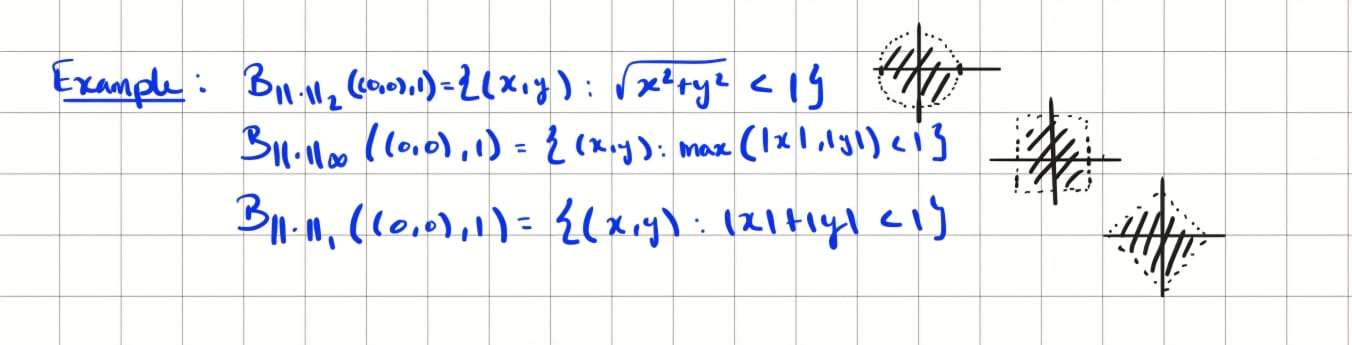
\includegraphics[width=\linewidth]{images/ball_example.jpeg}

\captionof{figure}{Example of the unit circle under different norms}
\end{example}



\section{Open and Closed sets}
\begin{definition}
    $X$ is a set. A \emph{Metric} $d$ is a map\[
    d: X \times X \to \R
    \]
    such that \begin{enumerate}
        \item $d(x,y) \ge 0$ with equality if and only if $x=y$.
        \item $d(x,y) = d(y,x)$.
        \item $d(x,z) \le d(x,y) + d(y,z)$.
    \end{enumerate}
\end{definition}
\begin{example}
    \begin{itemize}
        \item $(\R, |\cdot|)$
        \item Given a vector space $V$ with a norm $\cnorm$ we can define the metric $d(x,y) = ||x-y||$
        \item On any set $X$ the discrete metric is defined as \[
        d(x,y) = \begin{cases}
        0 & \text{if } x = y \\
        1 & \text{if } x \neq y
        \end{cases}
        \]
    \end{itemize}
\end{example}
\begin{question}
    Given a vector space $V$ with a metric $d$ on $V$ is $d$ coming from a norm? (i.e is there a norm $||\cdot||$ on $V$ such that $d(x,y) = ||x-y||$?)
    \textbf{Answer:} No, example let $(\R, d_{disc})$ suppose $\exists \cnorm$ such that $d(a,b) = ||a-b||$ then $d(2,0) = || 2-0|| = ||2|| = 1$ and $d(4,0) = ||4-0|| = ||4|| = 1$ but by the properties of a norm we have $||4|| = ||2\cdot 2|| = 2||2|| = 2\cdot 1 = 2$ contradiction.
\end{question}

\begin{notation}
    Given $(X,d)$ metric space, $ \delta >0$, and $x_0 \in X$ the $\delta$-neighborhood centered at $x_0$ is defined as \[
    N_{\delta}(x_0) = \{x \in X : d(x,x_0) < \delta \}  
    \]
\end{notation}

\begin{definition}
    $(X,d)$ metric space, $E \subseteq X$ \begin{itemize}
        \item $x_0 \in X$ is an \emph{interior point} of $E$ if and only if $\exists \delta >0$ such that $N_{\delta}(x_0) \subseteq E$.
        \item $x_0 \in X$ is a \emph{limit point} of $E$ if and only if $\forall \delta >0$ $N_{\delta}^*(x_0) \cap E \neq \emptyset$. We denote the set of limit points of $E$ as $E'$.
        \item $E$ is open if and only if every point of $E$ is an interior point.
        \item $E$ is closed if and only if $E' \subseteq E$
        \item The closure of $E$ is defined as $\overline{E} = E \cup E'$
    \end{itemize}
\end{definition}
\begin{example}
    $E = (0,1]$ in $(\R, |\cdot|)$ \begin{itemize}
        \item $E' = [0,1]$ and so $E$ is not closed
        \item The set of interior points of $E$ is $(0,1)$ so $E$ is not open since $1\in E$ but $1$ is not an interior point.
        \item $\overline{E} = E \cup E' = [0,1]$
    \end{itemize}
\end{example}

\paragraph{\bf Review at home} Make sure you know how to prove the following, you may refer to Rudin Chapter 2.
\begin{itemize}
    \item $N_{\delta}(x_0)$ is open $\forall x_0 \in X, \delta >0$.
    \item $E$ is open $\iff E^c$ is closed.
    \item $\overline{E}$ is closed in fact $\overline{E}$ is the smallest closed set containing $E$.
    \item Union of any collection of open sets is open.
    \item Finite intersection of open sets is open.
    \item Intersection of any collection of closed sets is closed.
    \item Finite union of closed sets is closed.
    \item If $x \in E'$ then $N_{\delta}(x) \cap E$ is infinite.
\end{itemize}
\begin{definition}
    Let $x_n$ be a sequence in $X$, we say that $x_n$ converges to $x_0 \in X$ if and only if $\forall \eps > 0$ $\exists N \in \N$ such that $d(x_n, x_0) < \eps$ $\forall n \ge N$. We denote this as $x_n \to x_0$.
\end{definition}

\begin{remark}\rm
    You could show as an exercise that in a metric space, the limit of a sequence, if it exists, is unique.

    Notice also from the definition that $x_n$ converges to $x_0$ in $(X,d)$ if and only if $d(x_n, x_0)$ converges to $0$ in $(\R, |\cdot|)$
\end{remark}


\begin{example}
    $x_n = (\frac{1}{n}+1, e^{-n})$ in $\R^2$ find the limit of $x_n$ in $(\R^2, ||\cdot||_{1})$ and $(\R^2, ||\cdot||_{2})$ and $(\R^2, ||\cdot||_{\infty})$.
    \paragraph{\bf Solution.}
        $x_0 = (1,0)$
        \[ ||x_n - x_0||_1 = \left|\left|\left(\frac{1}{n}, e^{-n}\right)\right|\right|_1 = \frac{1}{n} + e^{-n} \to 0 \]
        \[ ||x_n - x_0||_2 = \left|\left|\left(\frac{1}{n}, e^{-n}\right)\right|\right|_2 = \sqrt{\frac{1}{n^2} + e^{-2n}} \to 0 \]
        \[ ||x_n - x_0||_{\infty} = \left|\left|\left(\frac{1}{n}, e^{-n}\right)\right|\right|_{\infty} = \max\left\{\frac{1}{n}, e^{-n}\right\} \le \frac{1}{n}+e^{-n} \to 0 \]
        so in all 3 cases $x_n \to (1,0)$
\end{example}
\begin{proposition} 
    $x_n \to x_0$ in $(\R^k, ||\cdot||_{\infty}$) if and only if $x_{1,n} \to x_{1,0}, \dots , x_{k,n} \to x_{k,0}$ in $(\R, |\cdot|)$
    \begin{proof}
        We have for every $i=1,\cdots,k$
        
        $$0\leq |x_{i,n} - x_{i,0}| \le ||x_n - x_0||_{\infty}.$$
        and the forward direction follows.

        The converse follows as well from the following
        $$0\leq ||x_n - x_0||_{\infty}=\max\{|x_{1,n}-x_{1,0}|,\cdots, |x_{k,n}-x_{k,0}|\}\le |x_{1,n} - x_{1,0}| + \dots + |x_{k,n} - x_{k,0}|.$$
    \end{proof}
\end{proposition}

\begin{remark}
    $x \in \R^n$ \[ ||x||_{\infty} = \max(|x_1|, \dots, |x_n|) \le |x_1|+\dots +|x_n| = ||x||_1 \le n||x||_{\infty}\]
    \[ ||x||_{\infty} \le ||x||_1 \le n||x||_{\infty} .\]
\end{remark}
\begin{definition}
    Given a vector space $V$ and norms $||\cdot||_{a}$ and $||\cdot||_{b}$, we say that $||\cdot||_{a}$ and $||\cdot||_{b}$ are equivalent if and only if $\exists C_1, C_2 >0$ such that \[ C_1||x||_{b} \le ||x||_{a} \le C_2 ||x||_{b} \quad \forall x \in V \]
\end{definition}
\begin{example}
    $||\cdot||_{1}$, $||\cdot||_{\infty}$ are equivalent in $\R^n$ from the remark and you may also show that that $\|\cdot\|_\infty$ and $\|\cdot\|_2$ are equivalent.
\end{example}

\begin{remark}
    It is easy to check from the definition that each norm is equivalent to itself and that $\|\cdot\|_a$ and $\|\cdot\|_b$ are equivalent if and only if $\|\cdot\|_b$ and $\|\cdot\|_a$ are equivalent. Finally if $\|\cdot\|_a$, $\|\cdot\|_b$ are equivalent and $\|\cdot\|_b$,$\|\cdot\|c$ are equivalent then $\|\cdot\|_a$ and $\|\cdot\|_c$ are equivalent.
\end{remark}

\begin{lemma}
    $(X,d)$ metric space, $E \subseteq X$, $E$ is closed if and only if for every sequence $x_n$ in $E$ that converges, $\lim x_n \in E$
\begin{proof}
    $(\implies)$ Assume by contradiction that there exists a sequence $x_n \in E$ that converges to $x_0$ and $x_0 \notin E$. Take $\eps > 0$ then since $x_n \to x_0$ then $\exists N$ such that $x_n \in N_{\eps}(x_0)$ for $n \geq N$ so $N^*_{\eps}(x_0) \cap E \ne \emptyset \implies x_0 \in E'$ but E is closed so $E' \subseteq E$ contradiction.
    \\
    $(\impliedby)$ Let $x_0$ be in $E'$ take \[\eps = 1 \implies \exists x_1' \in N_{1}^*(x_0) \cap E\]
    \[\eps = \frac{1}{2} \implies \exists x_2' \in N_{\frac{1}{2}}^*(x_0) \cap E\]
    \[\vdots\]
    \[\eps = \frac{1}{n} \implies \exists x_n' \in N_{\frac{1}{n}}^*(x_0) \cap E\]
    So consider the constructed sequence $\{x_n\}$. We have $d(x_n, x_0) < \frac{1}{n}$ then $x_n \to x_0$ and by assumption $x_0 \in E$ so $E' \subseteq E$ thus $E$ is closed.
\end{proof}
\end{lemma}
\begin{example}
    $(0,1]$ is not closed in $(\R, |\cdot|)$ since $x_n = \frac{1}{n} \in (0,1]$ and $x_n \to 0 \notin (0,1]$
\end{example}

\begin{theorem}
    Given a vector space $V$ and norms $||\cdot||_a$ and $||\cdot||_{b}$ then the following are equivalent:
    \begin{enumerate}
        \item $||\cdot||_a$ and $||\cdot||_b$ are equivalent
        \item $x_n \to x_0$ in $(V, ||\cdot||_a)$ if and only if $x_n \to x_0$ in $(V, ||\cdot||_b)$
        \item $E$ is closed in $(V, ||\cdot||_a)$ if and only if $E$ is closed in $(V, ||\cdot||_b)$
        \item $G$ is open in $(V, ||\cdot||_a)$ if and only if $G$ is open in $(V, ||\cdot||_b)$
    \end{enumerate}
\end{theorem}
\begin{proof}
    \begin{itemize}
        \item $(1) \implies (2)$ $C_1\|x_n - x_0\|_b \le \|x_n -x_0\|_a \le C_2 \|x_n - x_0\|_b$ so $\|x_n - x_0\|_a \to 0 \iff \|x_n - x_0\|_b \to 0$
        \item $(2) \implies (3)$ by the previous lemma
        \item $(3) \implies (4)$ by complement
        \item $(4) \implies (1)$ $B_{\|\cdot\|_a}(0,1)$ open in $(V, \|\cdot\|_a)$ then it is open in $(V, \|\cdot\|_b)$. Hence $0$ is an interior point with respect to the $\|\cdot\|_b$ norm and so there  exists $\delta >0$ such that $$B_{\|\cdot\|_b}(0,\delta) \subseteq B_{\|\cdot\|_a}(0,1).$$
        Now let $x \in V$ with $x \ne 0$ then $ \frac{\delta}{2} \frac{x}{\|x\|_b} \in B_{\|\cdot\|_b}(0,\delta)\subseteq B_{\|\cdot\|_a}(0,1)$ so \[ \left\|\frac{\delta x}{2 \|x\|_b}\right\|_a < 1\implies \frac{\delta}{2\|x\|_b}\|x\|_a < 1\implies \|x\|_a < \frac{2}{\delta}\|x\|_b.\]
    \end{itemize}
    The inequality is trivial for $x=0$.
\end{proof}

\section{Compact Sets}
\begin{definition}
    Given a metric space $(X,d)$, we say that $K\subseteq X$ is \emph{compact} if and only if every open cover $\mathcal{G} = \{G_{\alpha} \}_{\alpha \in I}$ of $K$ (i.e. $K \subseteq \bigcup_{\alpha \in I} G_{\alpha}$) has a finite subcover $\{G_{\alpha_1}, \dots , G_{\alpha_n}\}$ such that $K \subseteq \bigcup_{i=1}^n G_{\alpha_i}$
\end{definition}

\begin{example}
    \begin{itemize}
        \item $(0,1]$ is not compact in $(\R, |\cdot|)$, since $\mathcal{G} = \{(\frac{1}{n}, 10) : n \in \mathbb{N}\}$ is an open cover but has no finite subcover.
        \item $[0, \infty)$ is not compact in $(\R, |\cdot|)$ since $\mathcal{G} = \{(-1,n) : n \in \N\}$ is an open cover but has no finite subcover
    \end{itemize}
\end{example}
\begin{example}
    If $K\subseteq X$ is finite then $K$ is compact
    \begin{proof}
        let $K = \{x_1, \dots, x_n \}$ and $\mathcal{G} = \{G_{\alpha}\}_{\alpha \in I}$ be an open cover of $K$ then $\forall x_i \in X$ $\exists G_{\alpha_i} \in \mathcal{G}$ such that $x_i \in G_{\alpha_i}$ so $K = \{x_1, \dots , x_n\} \subseteq G_{\alpha_1}\cup \dots \cup G_{\alpha_n}$ is a finite subcover of $\mathcal{G}$
    \end{proof}
\end{example}

\begin{proposition}
    Let $(X,d)$ be a metric space, and let $K \subseteq X$ be compact; then every closed subset $E$ of $K$ is compact.
\end{proposition}





\begin{proof}
    Let $\mathcal{G} = \{G_{\alpha}\}_{\alpha \in I}$ be an open cover of $E$. $E \subseteq \bigcup\limits_{\alpha \in I} G_{\alpha}$ then
    $$ K \subseteq E \cup E^c \subseteq \left(\bigcup_{\alpha\in I} G_{\alpha}\right) \cup E^c$$ so $\mathcal{G} \cup \{E^c\}$ is an open cover of $K$; thus, by compactness it has a finite subcover $\{G_{\alpha_1}, \dots , G_{\alpha_n}, E^c\}$ such that $K \subseteq G_{\alpha_1} \cup \dots \cup G_{\alpha_n} \cup E^c$; therefore, $E \subseteq G_{\alpha_1} \cup \dots \cup G_{\alpha_n}$ thus $\{G_{\alpha_1}, \dots , G_{\alpha_n}\}$ is a finite sub-cover of $\mathcal{G}$ covering $E$ concluding that $E$ is compact. 
\end{proof}

\begin{proposition}\label{prop:CompactBolzano}
If $K\subset X$ compact then every infinite set $E\subseteq K$ has a limit point in $K$.

We say then that $K$ satisfies the Bolzano-Weierstrass property.
\end{proposition}

\begin{proof}
    Let $E \subseteq K$ be an infinite set, suppose $E' \cap K = \emptyset$. Take $x \in K$ then $x \notin E'$ so $\exists \delta_x >0$ such that $N_{\delta_x}^*(x) \cap E = \emptyset$. $\mathcal{G} = \{N_{\delta_x}(x)\}_{x\in K}$ is an open cover of $K$ so it has a finite subcover $N_{\delta_{x_1}}(x_1), \dots , N_{\delta_{x_n}}(x_n)$ such that \[ K \subseteq \bigcup_{i=1}^n N_{\delta_{x_i}}(x_i) \] but \[ E \subseteq K \subseteq \bigcup_{i=1}^n N_{\delta_{x_i}}(x_i) \implies E= \bigcup_{i=1}^n \left(N_{\delta_{x_i}}(x_i)\cap E\right)\subseteq \{x_1, x_2, \dots , x_n \}.\] A contradiction, since $E$ is infinite.
\end{proof}




\subsection{Sequential Compactness}
\begin{definition}
Let $(X,d)$ be a metric space, and let $x_n$ be a sequence in $X$. Let $\phi: \N \to \N$ to be a strictly increasing function, then we say that $b_n = x_{\phi(n)}$ is a \emph{subsequence} of $x_n$
\end{definition}

\begin{remark}
    Recall $x_n \to x_0$ if and only if every subsequence of $x_n$ converges to $x_0$
\end{remark}

\begin{definition}
    Let $(X,d)$ be a metric space, we say that $K\subseteq X$ is \emph{sequentially compact} if and only if every sequence in $K$ has a convergent subsequence with limit in $K$.
\end{definition}

\begin{proposition}\label{prop:23}
    Let $(X,d)$ be a metric space, and assume $K\subseteq X$ admits the Bolzano-Weierstrass property then $K$ is sequentially compact.
\end{proposition}
\begin{proof}
Let $x_n$ be a sequence in $K$. $E = \{x_n : n \in \N\}$ 
    \begin{itemize}
        \item Case $E$ is finite: $\exists$ infinitely many $n$ such that $x_n = x_0$ for some $x_0 \in E \implies \exists n_1 < n_2 < \dots$ such that $x_{n_k} = x_0$ $\forall k$ so the subsequence $x_{n_k} \to x_0 \in K$
        \item Case $E$ is infinite: by assumption $\exists x_0 \in E'\cap K$, then \[\text{take } \eps = 1 \text{ then } \exists n_1 \text{ such that } x_{n_1} \in N_1^*(x_0) \cap E\] \[\text{take } \eps = 1/2 \text{ then } \exists n_2 > n_1 : x_{n_2} \in N_{1/2}^*(x_0) \cap E \]\[\text{We construct } n_k > n_{k-1} \text{ such that } x_{n_k} \in N_{1/k}^*(x_0) \cap E\] so the subsequence $x_{n_k} \to x_0 \in K$.
    \end{itemize}
\end{proof}

\begin{corollary}
Every compact set is sequentially compact.
\end{corollary}

\begin{proof}
    This follows from Propositions \ref{prop:CompactBolzano}, and \ref{prop:23}
\end{proof}

\subsection{Complete sets}
\begin{definition}
    Given a sequence $x_n$. We say that $x_n$ is Cauchy if and only if $\forall \eps>0$ $\exists N \in \N$ such that $d(x_n, x_m) < \eps$ $\forall n,m \ge N$
\end{definition}

\begin{proposition}
    If $x_n$ converges, then $x_n$ is Cauchy
\end{proposition}
\begin{proof}
    Let $x_n \to x_0$ then $\forall \eps >0$ $\exists N$ such that $d(x_n, x_0) < \frac{\eps}{2}$ $\forall n \ge N$ then by the triangle inequality \[ d(x_n, x_m) \le d(x_n, x_0) + d(x_m, x_0) < \frac{\eps}{2} + \frac{\eps}{2} = \eps \quad \forall n,m \ge N\]
\end{proof}




\begin{remark}
    The converse is false. For example take $(\Q, |\cdot|)$ and $x_n$ a sequence that converges to $\sqrt{2}$ in $(\R, |\cdot|)$ then $x_n$ is Cauchy in $(\Q, |\cdot|)$ but does not converge in $(\Q, |\cdot|)$.
\end{remark}

\begin{definition}
    $(X,d)$ metric space, $K \subseteq X$, we say that $K$ is complete if and only if every Cauchy sequence in $K$ converges to a point in $K$.
\end{definition}

\begin{example}
    From Math 210; $(\R, |\cdot|)$ is complete.
\end{example}

\begin{proposition}
    $K$ is complete then $K$ is closed.
\end{proposition}
\begin{proof}
    Let $x_n$ be a sequence in $K$ that converges to $x_0 \in X$ then $x_n$ is Cauchy and $K$ is complete then $x_n$ converges in $K$ so $x_0 \in K$ so $K$ is closed.
\end{proof}
\begin{remark}
    The converse is false. Take $(\Q, |\cdot|)$ then $\Q$ is closed in itself but not complete.
\end{remark}

\begin{proposition}
    $(X,d)$ metric space, $K$ complete and $E \subseteq K$ closed then $E$ complete
\end{proposition}

\begin{proof}
    Let $x_n$ be a Cauchy sequence in $E$ so $x_n$ is Cauchy in $K$ which is complete then $x_n$ converges in $K$ but $E$ is closed then $\lim_{n\to \infty}x_n \in E$ and so $E$ is complete.
\end{proof}

\begin{theorem}
    Let $V$ be a finite dimensional inner product space then $V$ is complete with respect to the norm induced by the inner product.
\end{theorem}
\begin{proof}
    Let $S = \{v_1,v_2, \dots v_{\ell}\}$ be an orthonormal basis of $V$ and $x_n$ be a Cauchy sequence in $V$ then $$x_n = r_{1,n}v_1 + r_{2,n}v_2+ \dots + r_{\ell,n}v_{\ell}.$$ We have 
    $$|r_{1,m} - r_{1,n}| = | \langle x_m, v_1 \rangle - \langle x_n, v_1 \rangle | = |\langle x_m - x_n, v_1 \rangle| \le  \|x_m - x_n\| \cdot \|v_1\|=\|x_m-x_n\|.$$ 
    Let $\eps > 0$, since $x_n$ is Cauchy then $\exists N$ such that $\|x_n - x_m\| < \eps$ and so $r_{1,n}$ is Cauchy in $ \R$ and since $\R$ is complete $r_{1,n} \to r_1 \in \R$. 
    Repeat the same argument for $i=1,\cdots,\ell$ we get $r_{i,n} \to r_i \in \R$. 
    
    Let $x= r_1v_1+ \dots +r_nv_n$ then $$\|x_n-x\| = \|(r_{1,n} -r_1)v_1 + \dots + (r_{\ell,n} - r_{\ell})v_l\| \le |r_{1,n}-r_1|  + \dots + |r_{\ell,n} - r_{\ell}|\to 0,$$
    and so $x_n$ converges to $x$ concluding that $V$
 is complete.
 \end{proof}

\begin{corollary}\label{eq:fdcomplete}
In a finite dimensional inner product space,
$K \subseteq V$ is complete if and only if it is closed.
\end{corollary}
\begin{proof}
    The result follows from above Proposition and Lemma.
\end{proof}
\begin{lemma}
      Let $x_n$ Cauchy sequence and assume $x_n$ has a convergent subsequence $x_{n_k}$ then $x_n$ converges to the subsequential limit.
\end{lemma}

\begin{proof}
     Given $ \eps > 0$, since $\lim_{k \to \infty} x_{n_k} = x_0$ then there exists $K \in \N$ such that $d(x_{n_k}, x_0) < \eps/2$ for $k \ge K$. $x_n$ Cauchy then $\exists N \in \N$ such that $d(x_n,x_m) < \eps/2$ for $n,m \ge N$. 
     Since $n_k\to \infty$ then there exists $L$ such that $n_L\geq \max\{N,K\}$.
     
     Let $n \ge N$ then \[d(x_n, x_0) \le d(x_n, x_{n_L}) + d(x_{n_L}, x_0) < \frac{\eps}{2} + \frac{\eps}{2} = \eps\] so $x_n \to x_0$.
\end{proof}

\begin{proposition}\label{prop:sequentialimplycomplete}
    $(X,d)$ metric space, $K \subseteq X$ sequentially compact then $K$ is complete.
\end{proposition}

\begin{proof}
    Let $x_n$ be a Cauchy sequence in $K$. Since $K$ is sequentially compact then $x_n$ has a convergent subsequence that converges in $K$ then by the previous Lemma, $x_n$ converges in $K$.
\end{proof}



\subsection{Total Boundedness}
\begin{definition}
    $(X,d)$ metric space, $K \subseteq X$ bounded if and only if $\exists x_0 \in X$ and $R >0$ such that \[ K \subseteq N_R(x_0),\] and we say that a sequence $x_n$ is bounded if and only if the set $E = \{x_n : n \in \N\}$ is bounded.
\end{definition}
\begin{remark}
    Recall that Cauchy and Convergent sequences are bounded.
\end{remark}
\begin{definition}
    $(X,d)$ metric space, $K \subseteq X$ we say that $K$ is totally bounded if and only if $ \forall \eps > 0 $ $\exists x_1, x_2, \dots , x_n \in K$ such that \[ K \subseteq \bigcup_{i=1}^n N_{\eps}(x_i), \]
    that is for every $\eps>0$ $K$ can be covered by finitely many $\eps$-neighborhoods with centers in $K$.
\end{definition}
\begin{proposition}
    $K \subseteq X$ is totally bounded $\implies K$ is bounded.
\end{proposition}

\begin{proof}
    let $\eps = 1$ then $$K \subseteq \bigcup\limits_{i=1}^t N_1(x_i)$$ with $x_1, \dots, x_t \in K$. 
    
    Let $M=\max\{d(x_1,x_j):j=1,\cdots,t\}.$ For $x \in K$ then $x \in N_1(x_i)$ for some $ 1\le i \le t$ then $$d(x,x_1) \leq d(x,x_i) + d(x_i, x_1) < 1 +M,$$ so $K \subseteq N_{1+M}(x_1)$ concluding that $K$ is bounded.
\end{proof}

\begin{remark}
    The converse is false. For example in $(\R, d_{disc})$. $\R$ is bounded, $\R \subseteq N_2(0)$ but not totally bounded since for $\eps = 1/2$ since if it was then $\exists x_1, \dots , x_n$ such that $ \R \subseteq \bigcup\limits_{i=1}^n N_{1/2}(x_i)$ but $N_{1/2}(x_i) = \{x_i\}$ so $\R \subseteq \{x_1, \dots , x_n\}$ contradiction.
\end{remark}

\begin{proposition}\label{prop:seqimplytotally}
    $K\subseteq X$ is sequentially compact then $K$ is totally bounded
\end{proposition}

\begin{proof}
    Suppose not, then $ \exists \eps_0$ such that $K$ cannot be covered by finitely many $\eps_0$-neighborhoods with centers in $K$. 
    
    Take $x_1\in K$, then $\exists x_2 \in K \setminus N_{\eps_0}(x_1)$ and similarly $\exists x_3 \in K \setminus N_{\eps_0}(x_1)\cup N_{\eps_0}(x_2)$ and so recursively given $x_1,\cdots, x_{n-1}$,  $\exists x_n \in K \setminus \bigcup\limits_{i=1}^{n-1} N_{\eps_0}(x_i)$. 
    
    Notice that for $m\neq n$,  $d(x_n, x_m) \ge \eps_0$ then $x_n$ has no convergent subsequence contradiction.
\end{proof}

\begin{lemma}
    Every subset of a totally bounded set is totally bounded.
\end{lemma}
\begin{proof}
    Take $K \subseteq X$ totally bounded, $E \subseteq K$ and $\eps>0$. Then 
    \[K \subseteq N_{\eps/2}(x_1) \cup \dots \cup N_{\eps/2}(x_t)\]
    where $x_1, \dots , x_t \in K$. Ignore the neighborhoods that do not intersect $E$ and re-index, we take $x_1, \dots , x_{\ell}$ be the points such that $N_{\frac{\eps}{2}}(x_i) \ne \emptyset$. Note that
    \[ E \subseteq N_{\eps/2}(x_1) \cup \dots \cup N_{\eps/2}(x_\ell)\]
    Take $y_i \in N_{\eps/2}(x_i) \cap E$ then
    \[N_{\eps}(y_i) \supseteq N_{\eps/2}(x_i) \quad (\text{ by triangle inequality})\] 
    This implies \[E \subseteq N_\eps(y_1) \cup \dots \cup N_\eps(y_\ell)\]
    with $y_1,\cdots,y_{\ell}$ in $E$ concluding that $E$ \text{ is totally bounded}
\end{proof}

\begin{example}
    $E = [0,1]$ is totally bounded since compact $\implies$ $(0,1)$ is totally bounded.
\end{example}

\begin{proposition}\label{prop:final implication}
    $(X,d)$ metric space. If $K \subseteq X$ is complete and totally bounded then $K$ is compact.
\end{proposition}

\begin{proof}
    Assume $K$ is not compact then there exists $\mathcal{G} = \{G_{\alpha}\}_{\alpha \in I}$ an open cover of $K$ that has no finite subcover. Let $\eps = 1$, $K$ is totally bounded then $K$ can be covered by finitely many neighborhoods with centers in $K$ and radius $1$. So $\exists x_1 \in K$ such that $K_1 = N_1(x_1) \cap K$ cannot be covered by finitely many open sets in $\mathcal{G}$. From above Lemma, $K_1$ is totally bounded, so letting $\eps = 1/2 \quad \exists x_2 \in K_1$ such that $K_2 = N_{1/2}(x_2)\cap K_1$ cannot be covered by finitely many open sets in $\mathcal{G}$. 
    
    We then recursively construct a sequence of sets $K_n = N_{1/n}(x_n) \cap K_{n-1}$ with $K_0:=K$ and $x_n \in K_{n-1}$ such that $K_n$ cannot be covered by finitely many open sets in $\mathcal G$. 
    Notice that
    $$K_0 = K \supseteq K_1 \supseteq K_2 \supseteq \dots.$$ 
    
    We show that $x_n$ is Cauchy. Let $\eps >0$ then $\exists N$ such that $1/N < \eps/2$. Let $m,n \ge N+1$, $x_n \in K_{n-1} \subseteq K_N$ similarly $x_m \in K_{m-1} \subseteq K_N$ and $K_N = N_{1/N}(x_N) \cap K_{N-1}$ so
    \[d(x_m,x_n) \le d(x_m,x_N) +d(x_n,x_N) \le \frac{1}{N}+\frac{1}{N} = \frac{2}{N} < \eps.\]
    Then $x_n$ is Cauchy in $K$ so by completeness it converges to some $x_0$ in $K$. Since $\mathcal{G}$ is an open cover of $K$ $\exists \alpha_0 \in I$ such that $x_0 \in G_{\alpha_0}$ open so $\exists \eps_0$ such that $N_{\eps_0}(x_0) \subseteq G_{\alpha_0}$. $x_n \to  x_0$ then $\exists N$ such that $x_N \in N_{\eps_0/2}(x_0)$ and $1/N < \eps_0/2$ so \[ K_N \subseteq N_{1/N}(x_N) \subseteq N_{\eps_0}(x_0) \subseteq G_{\alpha_0}\], contradiction.
\end{proof}

We have then concluded the following classification of compact sets in a general metric space.

\begin{theorem}
In a metric space $(X,d)$, the following are equivalent:
\begin{itemize}
    \item $K$ is compact
    \item $K$ satisfies the Bolzano-Weierstrass property.
    \item $K$ is sequentially compact.
    \item $K$ is complete and totally bounded.
\end{itemize}
\end{theorem}

\begin{proof}
    This follows from Propositions \ref{prop:CompactBolzano}, \ref{prop:23}, \ref{prop:sequentialimplycomplete}, \ref{prop:seqimplytotally}. \ref{prop:final implication}.
\end{proof}

\subsection{Compactness in Finite Dimensional Inner Product Spaces}
\begin{proposition}
    Given a finite dimensional normed space $V$, let $S = \{v_1,v_2, \dots, v_n\}$ be a basis of $V$ then the cube \[ Q_S = \{r_1v_1+r_2v_2+ \dots r_nv_n: |r_i|\le R\}\] is compact.
\end{proposition}

\begin{proof}
    Let $x^k = r_{1,k}v_1+ \dots + r_{n,k}v_n$ be a sequence in $Q_S$. Note that $r_{1,k}$ is a sequence in $[-R,R]$ compact so sequentially compact, then $r_{1,k}$ has a convergent subsequence $r_{1,k_\ell}$. Now $r_{2,k_\ell} \in [-R,R]$ compact then it has a convergent subsequence $r_{2,k_{\ell_t}}$. Doing this n-times $\exists$ a subsequence $\{k_j\}$ such that $r_{1,kj}, \dots , r_{n,kj}$ converges to $r_1,\dots , r_n$. Let $x = r_1v_1+ \dots +r_nv_n$\[ \|x_0-x^{kj}\| \le |r_{1,kj} - r_1|\|v_1\|+ \dots + |r_{n,kj}-r_n|\|v_n\| \to 0\quad \text{as }j\to \infty.\] Then $x^{k_j} \to x$ then $Q_S$ is sequentially compact and so compact.
\end{proof}

\begin{theorem}
    Let $V$ be a finite dimensional inner product space $K \subseteq V$ compact if and only if $K$ is closed and bounded.
\end{theorem}

\begin{proof}
    $(\implies)$ follows from the fact that complete sets are closed and totally bounded sets are bounded.
    \\
    $(\impliedby)$ Since $K$ is closed and $V$ is finite dimensional then $K$ is complete.
    
    We also have that K is bounded then $K\subseteq B(0,R)$ for some $R>0$. Let $\alpha=\{v_1,\cdots,v_n\}$ be an orthonormal basis of $V$. Take $x\in K$, then
    $$x=r_1v_1+\cdots+r_nv_n,$$
    and so $$|r_i|=|\langle x,v_i\rangle|\leq \|x\|\leq R,$$ and so $K\subseteq Q_S$. From the previous proposition $Q_S$ is compact so totally bounded and hence $K$ is totally bounded.

    Being complete and totally bounded we conclude that $K$ is compact.
    
\end{proof}
\begin{proposition}
    In a finite dimensional inner product space $V$,
    $K$ is bounded if and only if it is totally Bounded
\end{proposition}

\begin{proof}
    $(\impliedby)$ Already done.
    \\
    $(\implies)$ bounded $\implies$ Since $K$ is bounded then as in the proof of the previous Theorem $K\subseteq Q_S$ for some cube. Now $Q_S$ is compact then totally bounded and so $K$ is totally bounded.
\end{proof}


\section{Continuous Functions}

\begin{definition}
    Given metric spaces $X$ and $Y$, let $E\subseteq X$ and consider a map $f: E\to Y$.
    
    For $x_0 \in E'$, we write  $$\lim_{x \to x_0}f(x) = y_0 \in Y$$ if and only if $\forall \eps >0 \quad \exists \delta > 0$ such that $f(x) \in N_{\eps}(y_0)$ for $x \in N_{\delta}^*(x_0) \cap E$, that is 
    $$d_X(f(x),y_0)<\eps \quad\forall x\in E, 0<d_X(x,x_0)<\delta.$$
\end{definition}


\begin{definition}
    $f: E \to Y$ continuous at $x_0 \in E$ if and only if $ \forall \eps >0  \quad \exists \delta >0$ such that $f(x) \in N_\eps (f(x_0))$ for $x \in N_{\delta}(x_0) \cap E$.
    
    Hence, $f$ continuous at $x_0$ if and only if $x_0$ is an isolated point or $x_0 \in E' \text{ and } \lim\limits_{x\to x_0} f(x) = f(x_0)$.

    We say that $f$ is continuous in $E$ if and only if it is continuous at every point in $E$.
\end{definition}

\begin{remark}
$\lim\limits _{x\to x_0} f(x) = y_0$ if and only if for every sequence $x_n$ that converges to $x_0$ the sequence $f(x_n)$ converges to $y_0$ and so $f$ is continuous at $x_0$ if and only if for every sequence $x_n$ converging to $x_0$ we have $f(x_n) \to f(x_0)$. 

This provides a sequential definition for continuity that could be used to show that if $f,g$ continuous at $x_0$ then $f+g, cf, fg, f/g (g \ne 0)$ are continuous 
\end{remark} 

\begin{example} Given
    $f(x,y) = \frac{xy}{x^2+y^2}$ we want to find \[ \lim_{(x,y)\to(0,0)}f(x,y)\] 

    Consider the sequence 
    $(x_n,y_n) = (1/n,0)$, notice that $(x_n,y_n)\to (0,0)$, and $f(x_n,y_n)=0\to 0$. 
    
    On the other hand, consider the sequence $(x_n,y_n) = (1/n,1/n)$ also converging to $(0,0)$, we have 
    
    \[f(x_n,y_n) = \frac{1/n \cdot 1/n}{(1/n)^2+(1/n)^2} = \frac{1/n^2}{2/n^2} = \frac{1}{2}\to \frac12.\] 
    
    Therefore, having constructed two sequences that converge to $(0,0)$ whose images have different limits, then
    $\lim_{(x,y)\to (0,0)}$ does not exist.
\end{example}
\begin{remark}\rm
Some useful inequalities:
    \begin{itemize}
        \item $x^2+y^2 \ge x^2$
        \item $x^2+y^2 \ge y^2$
        \item $x^2+y^2 \ge 2|xy|$
    \end{itemize}
\end{remark}

\begin{example}
    Given $f(x,y) = \frac{x^2y}{x^2+y^2}$ we want to find $\lim_{(x,y)\to(0,0)} f(x,y)$. Note that \[0 \le |f(x,y)|= \left|\frac{x^2y}{x^2+y^2}\right| \le |y|.\]  Since $\lim\limits_{(x,y) \to (0,0)} |y| = 0$ then $\lim\limits_{(x,y) \to (0,0)} |f(x,y)| = 0$ and so $\lim\limits_{(x,y) \to (0,0)} f(x,y) = 0/$
\end{example}

\begin{example}
    $(V, \|\cdot\|)$ normed space, the map $\varphi: V \to \R$ given by $$\varphi(x) = \|x\|,$$
    is continuous.

  Notice from the homework that
  $$|\varphi(x)-\varphi(y)|=\Big| \|x\|-\|y\| \Big|\leq \|x-y\|.$$
  Hence $\varphi$ is continuous, in fact it is Lipschitz continuous.
\end{example}

\begin{proposition}
    Given a map $f: X\to Y$ then the following are equivalent
    \begin{enumerate}
        \item $f$ is continuous.
        \item $f^{-1}(H)$ is closed in $X$ for every $H$ closed in $Y$.
        \item $f^{-1}(G)$ is open in $X$ for every $G$ open in $Y$.  
    \end{enumerate}
\end{proposition}

\begin{proof}
    $((1)\implies (2))$ 
    Let $x_n$ be a sequence in $f^{-1}(H)$ that converges to $x_0$. We have $f(x_n)$ is a sequence in $H$ which by continuity converges to $f(x_0)$ and since $H$ is closed then $f(x_0)\in H$ concluding that $x_0\in f^{-1}(H)$ and so $f^{-1}(H)$ is closed.

    $((2)\implies (3))$ Let $G$ open in $Y$ then $G^c$ is closed and so $f^{-1}(G^c)=[f^{-1}(G)]^c$ is closed in $X$ concluding that $f^{-1}(G)$ is open.

    $((3)\implies (1))$ 
    Let $x_0\in X$, and $\epsilon>0$. $N_{\eps}(f(x_0))$ is open in $Y$ and so $f^{-1}(N_{\eps}(f(x_0)))$ is open in $X$ and contains $x_0$, therefore there exists $\delta>0$ such that
    $N_{\delta}(x_0)\subseteq f^{-1}(N_\eps(f(x_0)))$, and so
    $$f(N_{\delta}(x_0))\subseteq N_{\eps}(f(x_0)),$$
    concluding that $f$ is continuous at $x_0$.
\end{proof}

\begin{example}
    \[E = \{(x,y) \in \R^2: y >x\} \text{ is open in } \R^2\]\[f: \R^2 \to \R\] defined by \[f(x,y) = y - x\] then $E = f^{-1}((0,\infty))$ and $(0,\infty)$ is open in $\R$ and $f$ is continuous so $E$ is open in $\R^2$.
\end{example}
\begin{example}
    \[f: X \to Y \text{ continuous }\] Consider the "c"-level set with $c \in Y$ \[E = \{x \in X: f(x) = c\} \text{ is closed in } X\] since \[E = f^{-1}(\{c\})\] and $\{c\}$ is closed in $Y$ and $f$ is continuous so $E$ is closed in $X$.
\end{example}
\begin{remark}
    From the above example we conclude that all level sets of continuous functions are closed. Like the sphere, the disk, the cylinder.
\end{remark}
\begin{remark}
    $V,W$ normed spaces, and $\|\cdot\|_a,\|\cdot\|_b$ equivalent norms on $V$ so $f: (V,\|\cdot\|_a) \to W$ is continuous if and only if $f: (V,\|\cdot\|_b) \to W$ is continuous. 
\end{remark}
\begin{remark}
    $V,W$ normed spaces, and $\|\cdot\|_a,\|\cdot\|_b$ equivalent norms on $W$ so $f: V \to (W,\|\cdot\|_a)$ is continuous if and only if $f: (V \to (W,\|\cdot\|_b)$ is continuous. 
\end{remark}
\begin{proposition}
     Take $f: \R^m \to \R^n$ defined by \[f(x) = (f_1(x), f_2(x), \dots , f_n(x)) \qquad x= (x_1, x_2, \dots, x_m) \text{ is continuous}\] if and only if \[f:\R^m \to \R^n \text{ is continuous for every } 1 \le i \le n\]
\end{proposition}
    \begin{proof}
        The Euclidean norm and the infinity norm on $\R^n$ are equivalent.
    \end{proof}
\begin{theorem}[Extreme Value Theorem]
    $(X,d)$ metric space, $K \subseteq X$ compact, $f: K \to Y$ continuous then $f(K)$ is compact. In the special case where $Y = \R$ then f attains its maximum and minimum at a point in $K$.
\end{theorem}
\begin{proof}
    Using sequential compactness. Let $y_n$ be a sequence in $f(K)$ then $\exists x_n \in  K$ such that $f(x_n) = y_n$. Since $K$ is compact then $x_n$ has a convergent subsequence $x_{n_k}$ such that $x_{n_k} \to x_0 \in K$ then by continuity $y_{n_k} = f(x_{n_k}) \to f(x_0) \in f(K)$ so every sequence in $f(K)$ has a convergent subsequence in $f(K)$ so $f(K)$ is compact. 
    
    In the case where $Y = \R$, if $f(K)$ is compact in $\R$ so it is closed and bounded so  $\inf f(K)$, and $\sup(f(K))$ exist moreover they belong to $ \overline{f(K)} = f(K)$, since $f(K)$ is compact and so closed.
\end{proof}

\begin{theorem}
    All norms in a finite dimensional vector space are equivalent.
\end{theorem}

\begin{proof}
    $V$ is a finite dimensional vector space then by Problem set 1, we can define an inner product on $V$, and let $\|\cdot\|$ be the norm induced by our choice of inner product, and $S = \{v_1, \dots, v_n\}$ be an orthonormal basis of $V$. Let $\|\cdot\|_a$ be another norm on $V$ we will prove that $\|\cdot\|$ and $\|\cdot\|_a$ are equivalent. 
    
    Take $x \in V$ then \[x = r_1v_1 +\dots+ r_nv_n\] and \[|r_i| = |\langle x,v_i\rangle| \le \|x\|\cdot \|v_i\| = \|x\|.\] So \[\|x\|_a = \|r_1v_1+\dots+r_nv_n\|_a \le |r_1|\|v_1\|_a+\dots+|r_n|\|v_n\|_a \le (\|v_1\|_a+\dots+\|v_n\|_a)\|x\| = C_1\|x\| \quad \forall x \in V.\] 
    
    Now define the map $\varphi: (V, \|\cdot\|) \to \R$ $$\varphi(x) = \|x\|_a.$$ Note that $\varphi$ is continuous, in fact let $x_n \in V$ such that $x_n \to x_0$ in $(V, \|\cdot\|)$ then \[|\varphi(x_n) - \varphi(x_0)| = \Big|\|x_n\|_a - \|x_0\|_a\Big| \le \|x_n - x_0\|_a \le C_1\|x_n-x_0\| \to 0\] so \[\lim\limits_{n\to \infty}\varphi(x_n) = \varphi(x_0)\] concluding that $\varphi$ is continuous. 
    
    Let $K = \{x \in V: \|x\| = 1\}$ which is closed and bounded in the finite dimensional inner product space $(V, \|\cdot\|)$ then it is compact in $(V, \|\cdot\|)$ then by the extreme value theorem $\varphi(K)$ is compact in $\R$ so it attains its minimum in $K$. Notice that \[\varphi(x) = 0 \iff x = 0 \] and so for all $ x \in  K$, $ \varphi(x) >0$ which implies that  $\min(\varphi(K)) >0$. 
    
    Let $x \in V, x\ne 0$ then \[\frac{x}{\|x\|} \in K \implies \varphi\left(\frac{x}{\|x\|}\right) \ge \min(\varphi(K)) \implies \left\|\frac{x}{\|x\|}\right\|_a \ge \min(\varphi(K)) \implies \|x\|_a \ge \min(\varphi(K)) \|x\|:=C_2\|x\|.\]  
\end{proof}
\begin{corollary}
    In finite dimensional normed space, a set is compact $\iff$ closed and bounded regardless of the choice of norm.
\end{corollary}


\section{Connected sets}

\begin{definition}
    $(X,d)$ metric space, take $\Omega \subseteq X$ we say that $\Omega$ is disconnected if and only if there exists open sets $U,V \subseteq X$ such that $\Omega = (U \cup  V) \cap \Omega$ with $U \cap \Omega \ne \emptyset$ and $V \cap \Omega \ne \emptyset$ and $U\cap V\cap \Omega=\emptyset$. Otherwise, we say that $\Omega$ is connected.
\end{definition}

\begin{example}.
    \begin{itemize}
        \item  $\Om = (1,2] \cup (3,4)$ is disconnected.
        \item $\Q$ is disconnected in $\R$.
        \item 2 disjoint open balls in $\R^2$ are disconnected.
    \end{itemize}
\end{example}

\begin{proposition}
    $X$ is a connected metric space if and only if the only sets that are both open and closed in $X$ are $X$ and $\emptyset$.
\end{proposition}
\begin{proof}
    $(\implies)$ Assume that $U$ is open and closed and $U$ is not empty and $U \ne X$ then $U^c$ is closed and open and $U^c \ne \emptyset$ then $X = U \cup U^c$ then $X$ is disconnected.
    \\
    $(\impliedby)$ Assume that $X$ is disconnected then $X = U \cup V$ with $U,V$ non-empty,open and disjoint  then $V = U^c$ is both open and closed set, and $V \ne \emptyset$ and $V \ne X$.
\end{proof}

\begin{definition}
    $I \subseteq \R$ is an interval if and only if for $x,y \in I$ such that $x <y$ then $z \in I$ $\forall x < z<y$.
\end{definition}

\begin{example}.
    \begin{itemize}
        \item $(-\infty, 1]$
        \item $[1,2)$
        \item $[2,3]$
        \item $\Q$ is not an interval in $\R$ since $0,1 \in \Q$ but $\frac{1}{\sqrt{2}} \notin \Q$
    \end{itemize}
\end{example}

\begin{theorem}
    $\Om \subseteq \R$ is connected if and only if $\Om$ is an interval, i.e. the only connected sets in $\R$ are intervals.
\end{theorem}

\begin{proof}
    $(\implies)$ Assume $\Om$ is not an interval so $\exists x,y \in \Om$ and $z \notin \Om$ such that $x<z<y$ so $$\Om \subseteq (-\infty, z) \cup (z, \infty)$$ and hence $\Om$ is disconnected.

    
    $(\impliedby)$ Let $\Om$ be an interval, suppose $ \Om$ is not connected then $ \exists U,V$ open in $\R$ such that $$ \Om \subseteq U \cup V,\quad U \cap V \cap \Om = \emptyset\quad U \cap \Om, V \cap \Om \ne \emptyset.$$
    
    Take $x \in U \cap \Om$ and $ y \in V \cap \Om$ and assume without loss of generality, $x <y$. Since $\Omega$ is an interval then $[x,y] \subseteq \Om$.

    Let 
    $$z = \sup\set{[x,y] \cap U}.$$ 
    Since $[x,y] \cap U \ne \emptyset$ (it has $x$), and bounded above by $y$ then the supremum $z$ exists and $x\leq z\leq y$
    
    
    
    Assume $z\in U$, then $z<y$ (since $y\in V$). We then deduce that there exists $\delta>0$ such that $$(z,z+\delta)\subseteq U\cap [x,y],$$
    a contradiction by the definition of the supremum.
    
    Assume $z\in V$, then $z>x$ (since $x\in U$). We then deduce that there exists $\delta>0$ such that $$(z-\delta,z)\subseteq V\cap [x,y].$$
    By the definition of the supremum, there exists $z-\delta<z^*<z$ such that $z^*\in U\cap [x,y]$, a contradiction since $U\cap V\cap \Omega=\emptyset.$

    We get a contradiction as $z\in \Omega$, but $z\notin U\cup V,$ hence $\Omega$ is connected.
    
    
    
\end{proof}


\begin{theorem}[Intermediate value theorem]
    Given $f: X \to  Y$ continuous, if $X$ is connected then $f(X)$ is connected. In particular, if $Y = \R$ we have the following:\[ \text{ if } y_0,y_1 \in f(X) \text{ with } y_0\leq y_1\implies \forall \alpha \text{ such that } y_0 < \alpha < y_1 \text{ we have } f^{-1}(\alpha) \ne \emptyset\]
\end{theorem}
\begin{proof}
    Suppose $f(X)$ is disconnected, then $ \exists U,V$ open in $Y$ separating $f(X)$, then \[f(X) = (U \cup V) \cap f(X).\] Also note that \[ X = f^{-1}(f(X)) = f^{-1}((U\cup V) \cap f(X)) = f^{-1}(U) \cup f^{-1}(V).\] 
    
    Since $U$ and $V$ are open and $f$ is continuous so $f^{-1}(U)$ and $f^{-1}(V)$ are open in $X$, and \[f^{-1}(U) \cap f^{-1}(V) = f^{-1}(U \cap V) = \emptyset,\]
    moreover since $U \cap f(X) \ne \emptyset$ then $f^{-1}(U \cap f(X)) \ne \emptyset$ and similarly $f^{-1}(V) \ne \emptyset$, obtaining then that $X$ is disconnected.
    
    In the case when $Y =\R$, $f(X)$ is connected in $\R$ implies $f(X)$ is an interval and the result follows.
\end{proof}

\subsection{Path-connected Sets}
\begin{definition}
    $X$ is path connected if and only if $\forall a,b \in  X$ there exists a continuous function (path) \[\alpha: [0,1] \to X\] such that \[\alpha(0) = a \text{ and } \alpha(1) = b\] i.e every 2 points can be joined by a continuous path without leaving the set.
\end{definition}

\begin{remark}
    Given a vector space $V$, and $E\subseteq V$ if for $a,b \in V$ the line segment \[\{(1-t)a + tb : t \in [0,1]\} \subseteq X\] then $E$ is called convex.

    Clearly convexity is a special case of path connected.
\end{remark}

\begin{example}
    In a normed space $V$, the ball $B(x_0, R)$ is convex and hence path connected.
    \begin{proof}
        $a,b \in B(x_0, R) \implies \|x_0 -a\|, \|x_0-b\| < R$ then $$\| (1-t)a+tb -x_0\| = \|(1-t)a+tb-(1-t)x_0 - tx_0\| \le (1-t)\|a-x_0\|+t\|b-x_0\| < (1-t)R + tR = R$$ so the line segment from $a$ to $b$ is in $B(x_0,R)$.
    \end{proof}
\end{example}

\begin{proposition}
    $(X,d)$ metric space, if $X$ is path connected then $X$ is connected.
\end{proposition}

\begin{proof}
    Suppose $X$ is disconnected, then $X = U \cup V$ with $U,V$ open disjoint non-empty sets. Take $a \in U$ and $b \in V$, $X$ is path connected then $\exists \alpha: [0,1] \to X$ continuous such that $\alpha(0)=a$ and $\alpha(1) = b$. 
    Now 
    $$[0,1] = \alpha^{-1}(X) = \alpha^{-1}(U) \cup \alpha^{-1}(V)$$
    with $\alpha^{-1}(U)$ and $\alpha^{-1}(V)$ open disjoint non-empty sets contradicting the connectedness of $[0,1]$.
\end{proof}

\begin{theorem}
    $V$ vector space, $ \Om \subseteq V$ open, $\Om$ is connected if and only if $\Om$ is path connected.
\end{theorem}


\begin{remark}
    In Problem set 3, we  define the relation $R$ on $E\subseteq X$, as follows $aRb \iff \exists \alpha : [0,1] \to X$ continuous such that $\alpha(0) = a$, $\alpha(1) = b$ and $\alpha([0,1]) \subseteq E$ and prove $R$ is an equivalence relation.
\end{remark}

\begin{theorem}
    $(V, \|\cdot\|)$ normed space, $\Om \subseteq V$ open then $\Om$ connected if and only if $\Om$ path connected.
\end{theorem}

\begin{proof}
    $(\impliedby) $ done.
    \\
    $(\implies)$ Let $x_0 \in \Om$ \[A = \{y \in \Om: \exists \text{ path } \alpha \text{ joining } y \text{ to } x_0\}\] $A$ is open by Problem Set 3. $A \ne \emptyset$: $x_0 \in A$ and $\alpha:[0,1] \to V$ such that $\alpha(t) = x_0$. 
    
    
    Now take $B=\Omega\setminus A$. If $x\in B$, then since $\Omega$ is open there exists $\delta>0$ such that $B(x,\delta)\subseteq \Omega$. Now $B(x,\delta)$ is convex so no point in $B(x,\delta)$ can be joined to $x_0$ otherwise the center $x$ could be joined to $x_0$ which would imply that $x_0\in B$. Hence $B(x,\delta)\subseteq B$.

    We get that $\Omega=A\cup B$ with $A$ and $B$ open and disjoint, which is not possible unless $A$ or $B$ is empty but $A\neq \emptyset$ then $B=\emptyset$ obtaining that $\Omega=A$, and so every point in $\Omega$ can be joined to $x_0$ and so $\Omega$ is path-connected.
    
\end{proof}

\subsection{The topologist sine}
    Take the topological sine, $\Om = \{ (x, \sin(\frac{1}{x})): x > 0\} \cup \{(0,0)\}$. We want to prove it's connected but not path connected.
    
    In Problem Set 3, we show that that if $A$ is connected and $A \subseteq B \subseteq \overline{A}$ then $B$ is connected. 
    Take 
    $A = \{(x, \sin(\frac{1}{x})): x > 0\}$ connected. Take $f:(0,\infty) \to \R^2$ which is defined as $x \to (x, \sin(\frac{1}{x}))$ continuous and $(0,\infty)$ connected then $A = f((0,\infty))$ is connected by IVT. Hence since $$\Omega\subseteq\overline{A} = A \cup (\{0\} \times [-1,1])$$ so $\Om $ is connected.
    
    
    Next we show that $\Omega$ is not path-connected. Take $x_0 > 0$ and $(x_0, \sin(\frac{1}{x_0})) \in \Om$, suppose $\exists$ path $\alpha: [0,1] \to \Om$ continuous such that $\alpha(0) = (0,0)$ and $\alpha(1) = (x_0, \sin(\frac{1}{x_0}))$. 
    
    We write $\alpha(t) = (x(t),y(t))$. Let $t^* = \sup\{ t: x(t) = 0\}$ then by continuity $x(t^*) = 0$ then $t^* <1$ so $\alpha(t^*) = (0, 0)$. 

    We have $x(t^*)=0$ and $x(t)>0$ for $t\in (t^*,1)$ then letting $\eps = 1$ by IVT on $x(t)$ there exists $t^*<t_1 < t^*+1 \text{ with } t_1\in [0,1]$ such that \[x(t_1) = \frac{1}{(4n_1+1)\frac{\pi}{2}}\]
    for some $n_1\geq 1$ in $\mathbb N$.
    
    Now take $\eps = \frac{1}{2}$ then again by IVT on $x(t)$ $\exists t^* < t_2 < t^* + \frac{1}{2}$ such that \[x(t_2) = \frac{1}{(4n_2+1)\frac{\pi}{2}},\]
    for some $n_2\geq 2$ integer.
    
    Recursively, for every $k\in \mathbb N$, there exists sequence $t_k \in [0,1]$ with $t^* < t_k < t^*+\frac{1}{k}$ such that \[x(t_k) = \frac{1}{(4n_k+1)\frac{\pi}{2}}\] 
    with $n_k\geq k$ in $\mathbb N$.
    
    We have \[\alpha(t_k) = \left(\frac{1}{(4n_k+1)\frac{\pi}{2}}, \sin\left[(4n_k+1)\frac{\pi}{2}\right)\right]=\left(\frac{1}{(4n_k+1)\frac{\pi}{2}},1\right).\] 
    Letting $k\to \infty$, $t_k\to t^*$ and $n_k\to \infty$ and so by continuity of $\alpha$ we get that $$\alpha(t^*) = (0,1),$$ a contradiction. Therefore, the topologist sine is not path connected.





\begin{figure}[h!]
    \centering
    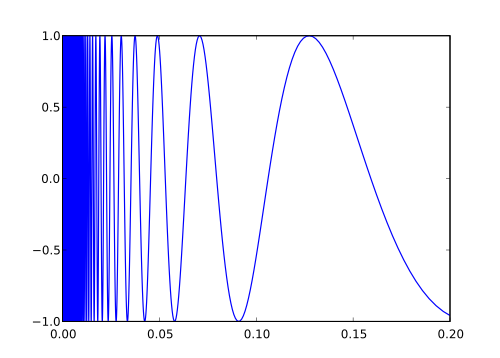
\includegraphics[width=0.75\linewidth]{images/Topologist's_sine_curve.svg.png} 
    \caption{Topologist's sine curve}
    \label{fig:sample_image} 
\end{figure}

\chapter{Differentiation}
\section{Review of Linear Transformations}
\begin{definition}
    $T: V \to W$ is a linear transformation if and only if $T(v_1+\alpha v_2) = Tv_1+\alpha Tv_2 \quad \forall v_1, v_2 \in V \text{ and } \alpha \in \R$.
\end{definition}
\begin{notation}
\begin{itemize}
    \item For a basis $\alpha=\{v_1,v_2,\cdots,v_n\}$ of $V$, and $v\in V$ there exists unique $r_1,\cdots,r_n$ such that $v=r_1v_1+r_2v_2+\cdots+r_nv_n$. We denote by
    $$[v]_\alpha=\begin{pmatrix} r_1\\ r_2\\ \vdots \\ r_n\end{pmatrix}.$$
    $[\cdot]_{\alpha}$ is in fact an isomorphism from $V$ to $\mathbb R^n$.
    \item We denote by $\mathcal{L}(V,W)$ the space of linear transformations from $V$ to $W$. $\mathcal{L}(V,W)$ is a vector space. If $\dim(V) = n$ and $\dim(W) = m$ then $\dim\mathcal{L}(V,W) = mn$. For $\alpha = \{v_1, \dots, v_n\}$ and $\beta = \{w_1, \dots , w_m\}$ bases of $V$ and $W$ respectively, we can represent $T$ uniquely by an $m \times n $ matrix \[ [T]_{\alpha}^{\beta} = ([Tv_1]_\beta|[Tv_2]_\beta| \quad \dots \quad |[Tv_n]_\beta).\] In fact, $[\cdot]_{\alpha}^\beta:T\mapsto [T]_{\alpha}^\beta$ is an isomorphism from $\mathcal L(V,W)$ to $M_{m\times n}(\mathbb R)$.
    We also have
    $$[Tv]_{\beta}=[T]_{\alpha}^{\beta}[v]_{\alpha}.$$
    This notation justifies identifying matrices with linear transformations.
    \item In the particular case when $V=\mathbb R^n$, and $W=\mathbb R^m$, and $T\in \mathcal L(\mathbb R^n,\mathbb R^m)$, $[T]$ corresponds to the associated matrix with respect to the standard Euclidean bases.
\end{itemize}
\end{notation}

\begin{proposition}
    Let $V$ and $W$ be normed spaces, and let $T: V \to W$ be a linear transformation, then the following are equivalent: \begin{enumerate}
        \item $T$ is continuous on $V$
        \item $T$ is continuous at $0$
        \item $\exists M>0 \text{ s.t } \|Tx\|_W \leq  M \|x\|_V \quad \forall x \in V $
    \end{enumerate}
\end{proposition}

\begin{proof}
    $(1) \implies (2)$ done.\\
    $(2) \implies (3)$. $T$ is continuous at 0, then for $\eps =1$ there exists $\delta >0$ such that, $\|Tx -T0\|_W < 1$ for all $x$ such that $\|x-0\|_V < \delta$. Since $T0=0$ then $\|Tx\|_W< 1$ for $\|x\|_V < \delta$. Take any $x \ne 0$, $\left\|\frac{\delta x}{2\|x\|_V}\right\|_V = \frac{\delta}{2}<\delta$ so \[\left\|T\left(\frac{\delta x}{2\|x\|_V}\right)\right\|_W < 1\] concluding that $\|Tx\|_W\leq \dfrac{2}{\delta}\|x\|_V.$\\
    $(3) \implies (1).$ $\|Tx-Ty\|_W = \|T(x-y)\|_W \le M\|x-y\|_V$ so $T$ is Lipschitz continuous.
\end{proof}
\begin{theorem}
    If $V$ is a finite dimensional normed space then every linear transformation $T:V\mapsto W$ is continuous.
\end{theorem}

\begin{proof}
    Since all norms on $V$ are equivalent, we consider a norm on $V$ induced by an inner product and we let $\alpha=\{v_1,v_2,\cdots,v_n\}$ be an orthonormal basis of $V$. Let $x\in V$, then $x=r_1v_1+\cdots+r_nv_n$ for some $r_i\in \mathbb R$, and by Cauchy Schwarz 
    $$|r_i|=|\langle x,v_i\rangle|\leq \|x\|_V.$$
    Hence by linearity
    $$\|Tx\|_W=\|r_1Tv_1+\cdots+r_n Tv_n\|_{W}\leq |r_1|\|Tv_1\|_W+\cdots+|r_n|\|Tv_n\|_W\leq \left(\|Tv_1\|_W+\cdots+\|Tv_n\|_W\right) \|x\|_V.$$

\end{proof}

\begin{example}
    Above result is not true if $V$ is not finite dimensional. For example let $C^1([0,1])$ the space of continuously differentiable functions and $C([0,1])$ the space of continuous functions. We consider the sup norms on both spaces. The differentiation operator 
    $\dfrac{d}{dx}\in \mathcal L(C^1([0,1]), C([0,1]))$ is not continuous. In fact, assume it is then by above proposition there exists $M$ such that 
    $$\left\|\dfrac{d}{dx}f\right\|_\infty\leq M \|f\|_{\infty}.$$
    Let $f_n=x^n$ on $[0,1]$. We have $\|f_n\|_{\infty}=1$ and $\|f_n'\|_{\infty}=\|nx^{n-1}\|_{\infty}=n.$
    Hence, replacing we obtain for every $n\in \mathbb N$
    $n\leq M$, a contradiction.
\end{example}

\section{Differentiability of functions}
\paragraph{\bf Convention.} 
Given vectors $u,v\in \mathbb R^n$, we define
$$u\cdot v=\sum_{i=1}^n u_iv_i.$$
This definition is independent of whether we write vectors as row or column matrices.

If we represent vectors as column matrices, then
\[
u\cdot v = u^{t}v.
\]


\begin{definition}[little oh]
    Let $r:V\mapsto W$ be a function defined in a neighborhood of $0$. We say that $r(h)$ is little-oh of $h$ and write $r(h)=o(\|h\|)$ as $h\to 0$ if and only if for every $\epsilon>0$ there exists $\delta>0$ such that 
    $$\|r(h)\|_{W}\leq \epsilon \|h\|_{V}\qquad \forall \|h\|_V<\delta,$$ equivalently
    $$\lim_{h\to 0}\dfrac{\|r(h)\|_W}{\|h\|_V}=0.$$
\end{definition}
\paragraph{\bf Motivation.} In $1$-dimension, for $f: \R \to \R$, we say that $f$ is differentiable at $x_0$ if and only if
    \begin{align*}
    \lim_{h\to 0} \frac{f(x_0+h) - f(x_0)}{h}, \quad \text{or equivalently} \lim_{x\to x_0} \dfrac{f(x)-f(x_0)}{x-x_0}
    \end{align*}
    exists.
    If the limit exists we denote it by $f'(x_0)$.

    Notice that
    \begin{align*}
    L = \lim_{x \to x_0}\frac{f(x)-f(x_0)}{x-x_0} &\iff \lim_{x\to x_0}\left(\frac{f(x)-f(x_0)}{x-x_0}-L\right) = 0 \\
    &\iff \lim_{x\to x_0} \frac{f(x)-f(x_0)- L(x-x_0)}{x-x_0} = 0\\
    &\iff \exists L \in \R \text{ s.t } f(x) = f(x_0)+L(x-x_0) + o(|x-x_0|)
    \end{align*}

\begin{definition}
    Let $V$ and $W$ be normed spaces, $U$ be an open subset of $V$, and $x_0 \in U$, we say that $f$ is differentiable if and only if there exists a continuous linear transformation $T\in \mathcal{L}(V,W)$ such that \[f(x) = f(x_0)+T(x-x_0) + o(\|x-x_0\|),\qquad \text{or equivalently}\quad  f(x_0+h) = f(x_0)+T(h)+o(\|h\|)\]  if and only if \[ \exists T \in \mathcal{L}(V,W) \text{ such that} \lim_{h \to 0}\frac{\|f(x_0+h) - f(x_0) - T(h)\|_W}{\|h\|_V} = 0\]
\end{definition}

\begin{proposition}
        If such a $T$ exists then it is unique.
\end{proposition}

\begin{proof}
Suppose $\exists T_1, T_2$ continuous linear transformations in $\mathcal{L}(V,W)$ such that \[f(x_0+h) = f(x_0)+T_1(h)+o_1(\|h\|),\qquad \text{and}\qquad f(x_0+h) = f(x_0)+T_2(h)+o_2(\|h\|)\] so subtracting we get \[(T_2-T_1)(h) = o_3(\|h\|).\] 
Take $v\in V$ such that $\|v\| = 1$ so for every $\lambda\in \mathbb R$,
\[(T_2-T_1)(\lambda v) =\lambda(T_2-T_1)(v) = o_3(|\lambda|)\] so \[(T_2-T_1)(v) = \frac{o_3(|\lambda|)}{\lambda}\to 0 \text{ as $\lambda\to 0$}.\] Hence $(T_2 - T_1)(v) = 0$ for every $\|v\|=1$ implying that $T_2 = T_1$.
\end{proof}

\begin{definition}
    If $f$ is differentiable at $x_0$ then we let $Df(x_0)$ be the continuous linear transformation in $\mathcal{L}(V,W)$ such that \[f(x) = f(x_0)+Df(x_0)(x-x_0)+ o(\|x-x_0\|) \iff 
    f(x_0+h) = f(x_0)+Df(x_0)(h)+ o(\|h\|)
    \]
    \[\iff
    \lim_{x\to x_0}\frac{\|f(x)-f(x_0)-Df(x_0)(x-x_0)\|_W}{\|x-x_0\|_V} = 0\]
\end{definition}

\begin{remark}
We note the following:
\begin{itemize}
    \item We will consider mostly finite dimensional vector spaces and so all linear transformations are continuous in that case.
    \item In case $V=\mathbb R^n$, and $W=\mathbb R^m$, the $m\times n$ matrix associated to the derivative linear transformation is called the Jacobian matrix. In that case, we have
    $$f(x_0+h)=f(x_0)+[Df(x_0)]h+o(\|h\|).$$
    Here $h$ is considered to be a column vector in $\mathbb R^n$. In fact, when we write in matrix forms, we represent vectors in $\mathbb R^n$ as column vectors.
\end{itemize}
    
\end{remark}


\begin{example}
    In $1$ variable $[Df(x_0)] = [f'(x_0)]$ so $Df(x_0): t\in \mathbb R \mapsto f'(x_0) t$. 
\end{example}
\begin{example}
We find the derivative of $f(x,y) = x^2 + y^2$. \[f((x_0,y_0)+(h_1,h_2)) = f(x_0+h_1,y_0+h_2) = (x_0+h_1)^2+(y_0+h_2)^2 = x_0^2+y_0^2+2x_0h_1+2y_0h_2+h_1^2+h_2^2. \] Notice that \[\frac{h_1^2+h_2^2}{\sqrt{h_1^2+h_2^2}} \to 0\] and 
$$h\mapsto 2x_0h_1+2y_0h_2,$$
is in $\mathcal L(\mathbb R^2, \mathbb R)$, therefore $f$ is differentiable at $(x_0,y_0)$

\[Df(x_0,y_0): h \mapsto 2x_0h_1+2y_0h_2\] so the Jacobian matrix is $[Df(x_0,y_0)] = \begin{pmatrix}
        2x_0 & 2y_0
    \end{pmatrix}$
\end{example}
\begin{example}
    Let $T: V \to W$ be a continuous linear transformation. We have
    \[T(x_0+h) = T(x_0)+T(h)+0\implies DT(x_0) = T.\]
\end{example}

\begin{proposition}
    $f: V \to W$ differentiable at $x_0$ then $f$ is continuous at $x_0$.
\end{proposition}
\begin{proof}
    $f(x) = f(x_0)+Df(x_0)(x-x_0)+o(\|x-x_0\|)$.
    Notice that
    $$o(\|x-x_0\|) = \frac{o(\|x-x_0\|)}{\|x-x_0\|}\|x-x_0\| \to 0\quad \text{as $x\to x_0$}.$$ Since $Df(x_0)$ is continuous then 
    $$Df(x_0)(x-x_0)\to Df(x_0)(0)=0\quad \text{as $x\to x_0$}.$$
    Hence $\lim_{x\to x_0} f(x) = f(x_0)$ concluding that $f$ is continuous at $x_0$.
\end{proof}
\section{Partial Derivatives of real-valued functions}
In this section, we introduce partial derivatives of order $1$ for real-valued functions, allowing us to check more easily differentiability and calculate the derivative map.

\begin{definition}
    Let $U\subseteq \R^n$ be open, $f:U\to \R$, and $x_0\in U$. For $1\leq i\leq n$, the partial derivative of $f$ with respect to $x_i$ at $x_0$ is
    \[\frac{\partial f}{\partial x_i}(x_0) = \lim_{t \to 0} \frac{f(x_0+te_i)-f(x_0)}{t},\]
    if it exists.
    Here $e_i$ is the i-th standard basis in $\mathbb R^n$.
\end{definition}

\begin{remark}
    From the definition, the partial derivatives correspond to the one variable derivatives assuming all components except the i-th is constant. For example, if $f(x,y,z)=x^2+2y-xz$, then
    $$\dfrac{\partial f}{\partial x}=2x-z, \quad \dfrac{\partial f}{\partial y}=2,\qquad \dfrac{\partial f}{\partial z}=-x.$$
\end{remark}

\begin{example} The function
    \[f(x,y) = \begin{cases}
        \frac{xy}{x^2+y^2} & (x,y) \ne (0,0)\\
        0 & (x,y) = (0,0)
    \end{cases}\]
    is not continuous at $(0,0)$ and so not differentiable but the partial derivatives at $(0,0)$ exist. In fact
    $$\frac{\partial f}{\partial x}(0,0) = \lim_{t \to 0} \frac{f(t,0)-f(0,0)}{t} = 0,\qquad \frac{\partial f}{\partial y}(0,0) = \lim_{t \to 0} \frac{f(0,t)-f(0,0)}{t} = 0.$$
\end{example}

\begin{theorem}
    $U \subseteq \R^n$ open and $f: U \mapsto \R$ is differentiable if and only if all partial derivatives of order $1$ exist and \[\lim_{h\to 0} \frac{|f(x_0+h)-f(x_0)-\nabla f(x_0)\cdot h|}{|h|} = 0,\]
with $\nabla f(x_0)=\left(\dfrac{\partial f}{\partial x_1}(x_0),\cdots, \dfrac{\partial f}{\partial x_n}(x_0)\right),$
and so $Df(x_0)(h)=\nabla f(x_0)\cdot h.$
\end{theorem}

\begin{proof}
The backward direction follows from the definition of differentiability.

To prove the forward direction, assume $f$ is differentiable, and write
$$f(x)=f(x_0)+Df(x_0)(x-x_0)+o(|x-x_0|).$$
Hence
$$\dfrac{f(x_0+te_i)-f(x_0)}{t}=Df(x_0)(e_i)+\dfrac{o(|t|)}{t}\to Df(x_0)(e_i)\quad \text{as $t\to 0$}.$$
So all partial derivatives exist and $\dfrac{\partial f}{\partial x_i}(x_0)=Df(x_0)(e_i).$
Hence
$$Df(x_0)(h)=Df(x_0)(h_1e_1+\cdots+h_ne_n)=\sum_{i=1}^n h_iDf(x_0)(e_i)=\sum_{i=1}^n h_i\dfrac{\partial f}{\partial x_i}(x_0)=\nabla f(x_0)\cdot h.$$ 
\end{proof}

\begin{example}
Let's check whether $f(x,y) = \begin{cases}
        \frac{x^2y}{x^2+y^2} & (x,y) \ne (0,0)\\
        0 & (x,y) = (0,0)
    \end{cases}$ is differentiable at $(0,0).$ \[f_x(0,0) = \lim_{h_1 \to 0} \frac{f(h_1,0)-f(0,0)}{h_1} = 0\qquad f_y(0,0)=\lim_{h_2 \to 0} \frac{f(0,h_2)-f(0,0)}{h_2}=0.\]
    So partial derivatives of order $1$ exist at $(0,0)$, and $\nabla f(0,0)=(0,0)$. Next we check
    \[\frac{|f((0,0)+(h_1,h_2))-f(0,0)- \nabla f(0,0) \cdot (h_1,h_2)|}{\sqrt{h_1^2+h_2^2}} = \frac{h_1^2h_2}{(h_1^2+h_2^2)\sqrt{h_1^2+h_2^2}}, \] let $h_1 = \frac{1}{n}$ and $h_2 = \frac{1}{n}$ we get \[\frac{\frac{1}{n^3}}{\frac{2 \sqrt{2}}{n^3}} \to \frac{1}{2 \sqrt{2}} \quad \text{ as $n\to \infty$}.\] So above quantity does not go to zero (in fact the limit does not exist) and so $f$ is not differentiable.
\end{example}


\begin{example}
Let's check whether $f(x,y) = \begin{cases}
        \frac{x^2y^2}{x^2+y^2} & (x,y) \ne (0,0)\\
        0 & (x,y) = (0,0)
    \end{cases}$ is differentiable at $(0,0).$ \[f_x(0,0) = \lim_{h_1 \to 0} \frac{f(h_1,0)-f(0,0)}{h_1} = 0\qquad f_y(0,0)=\lim_{h_2 \to 0} \frac{f(0,h_2)-f(0,0)}{h_2}=0.\]
    So partial derivatives of order $1$ exist at $(0,0)$, and $\nabla f(0,0)=(0,0)$. Next we check
    \[\frac{|f((0,0)+(h_1,h_2))-f(0,0)- \nabla f(0,0) \cdot (h_1,h_2)|}{\sqrt{h_1^2+h_2^2}} = \frac{h_1^2h_2^2}{(h_1^2+h_2^2)\sqrt{h_1^2+h_2^2}}=\dfrac{h_1^2}{h_1^2+h_2^2}\times \dfrac{|h_2|}{\sqrt{h_1^2+h_2^2}}|h_2|\leq |h_2|\to 0.\] 
    Hence $f$ is differentiable at $(0,0)$.
\end{example}


\begin{example}
 Consider the function $f(x,y) = x \sqrt{y}$ with $x\in \mathbb R$ and $y\geq 0$.
 Notice that $\frac{\partial f}{\partial x} = \sqrt{y}$ for every $x\in \mathbb R$ and $y\geq 0$, and  $\frac{\partial f}{\partial y} = \frac{x}{2\sqrt{y}}$ for every $x\in \mathbb R$ and $y>0$.

 We shall show later that if partial derivatives exist in a neighborhood of a point and are continuous at that point then $f$ is differentiable. This implies that $f$ is differentiable at $(x,y)$ for every $x\in \mathbb R$ and $y>0$. You can also prove this fact above by using the definition.
 
What about at $(x,0)$? We have $\dfrac{\partial f}{\partial x}$ exists but 
    \[\lim_{h_2 \to 0} \frac{f(x,0+h_2)-f(x,0)}{h_2} = \lim_{h_2 \to 0} \frac{x \sqrt{h_2}}{h_2} = \lim\limits_{h_2 \to 0} \frac{x}{\sqrt{h_2}}\]
    \begin{itemize}
        \item if $x > 0$ and $y =0 $ then $\lim\limits_{h \to 0} \frac{x}{\sqrt{h}}$ doesn't exist and $\dfrac{\partial f}{\partial y}$ does not exist, and so $f$ is not differentiable at $(x,0)$ with $x>0$.
        \item if $x = 0$ and $y = 0$ then $\lim\limits_{h \to 0} \frac{0}{\sqrt{h}} = 0$ so $\frac{\partial f}{\partial y}(0,0) = 0$. Let's check differentiability
        $$\dfrac{|f((0,0)+(h_1,h_2))-f(0,0)-\nabla f(0,0)\cdot (h_1,h_2)|}{\sqrt{h_1^2+h_2^2}}=\dfrac{|h_1|\sqrt{h_2}}{\sqrt{h_1^2+h_2^2}}\leq \sqrt{h_2}\to 0\quad \text{as $(h_1,h_2)\to (0,0)$}.$$
    \end{itemize}
\end{example}

\begin{theorem}
    $U \subseteq \R^n$ and $f=(f_1,\cdots,f_m): U \to \R^m$ then $f$ is differentiable if and only if $f_i: U \to \R$ is differentiable for all $1 \le i \le m$.
    
    In this case, \[Df(x_0)(h)= \begin{pmatrix}
        \nabla f_1(x_0)\cdot h \\
        \nabla f_2(x_0)\cdot h \\
        \vdots \\
        \nabla f_m(x_0)\cdot h
    \end{pmatrix},\] and so 
    \[[Df(x_0)] = \begin{pmatrix}
    \nabla f_1(x_0)\\
    \nabla f_2(x_0)\\
    \vdots\\
    \nabla f_m(x_0)\end{pmatrix} = \begin{pmatrix}
    \dell{f_1}{x_1}(x_0) & \dots & \dell{f_1}{x_n}(x_0)\\
    \dell{f_2}{x_1}(x_0) & \dots & \dell{f_2}{x_n}(x_0)\\
    \vdots & \ddots & \vdots\\
    \dell{f_m}{x_1}(x_0) & \dots & \dell{f_m}{x_n}(x_0)
    \end{pmatrix} \]
\end{theorem}

\begin{example}
For $f(x,y) = (x^2y^2, x^2+y^2, x^2 - y^2).$ The function is differentiable and
$[Df(x,y)] = \begin{pmatrix}
    2xy^2 & 2x^2y\\
    2x & 2y\\
    2x & -2y
    \end{pmatrix}.$
For example at $(1,2)$, $[Df(1,2)] = \begin{pmatrix}
    8 & 4\\
    2 & 4\\
    2 & -4
    \end{pmatrix}$, and
  \[Df(1,2): h \mapsto \begin{pmatrix}
        8h_1 + 4h_2 \\
        2h_1 + 4h_2 \\
        2h_1 - 4h_2
    \end{pmatrix}\]
\end{example}

\begin{proof}
    $(\implies)$ Assume $f$ is differentiable at $x_0$ then \[f(x_0+h)= f(x_0)+Df(x_0)(h) + o( \|h\|).\] Dotting with $e_i\in \mathbb R^m$ we get \[f_i(x_0+h) = f_i(x_0)+ Df(x_0)(h)\cdot e_i+ o(\|h\|)\cdot e_i\] and $\frac{o(\|h\|)\cdot e_i}{\|h\|} \to 0.$ Therefore $f_i$ is differentiable for every $i$ and $Df_i(x_0): h \mapsto Df(x_0)(h) \cdot e_i$\\
    $(\impliedby)$ Assume all $f_i$ are differentiable then \[f_i(x_0+h) = f_i(x_0)+Df_i(x_0)(h)+ o_i(\|h\|)\] and so
    \begin{align*}
        f(x_0+h) &= f(x_0)+(Df_1(x_0)(h), \cdots, Df_m(x_0)(h))+(o_1(\|h\|), \cdots, o_m(\|h\|))\\
        &=f(x_0)+(\nabla f_1(x_0)\cdot h, \cdots, \nabla f_m(x_0)\cdot h)+(o_1(\|h\|), \cdots, o_m(\|h\|)).
    \end{align*} 

    Notice that $\lim_{h\to 0}\dfrac{(o_1(\|h\|), \cdots, o_m(\|h\|))}{\|h\|}=0$ and so $f$ is differentiable at $x_0$ and \[Df(x_0): h \mapsto  (
        \nabla f_1(x_0)\cdot  h,
        \nabla f_2(x_0)\cdot h,
        \cdots,
        \nabla f_m(x_0)\cdot h)\]
\end{proof}

\begin{remark}
    If $f,g$ are differentiable then $f+ \alpha g$ is differentiable and $D(f+ \alpha g) = Df+ \alpha Dg$
\end{remark}
\begin{proof}
     Use the definition.
\end{proof}

\section{Chain Rule}

\begin{theorem}
    $U \subseteq \R^n$, $x_0\in U$ $f: U \to \R^m$. Let $V$ be an open subset of $\mathbb R^m$ containing $f(U)$, and assume $g:V\mapsto \mathbb R^k$. Define $h=g\circ f: U\mapsto \mathbb R^k$
    \[ " U \xrightarrow{f} f(U)\subseteq \R^m \xrightarrow{g} \R^k ."\] 
    If $f$ is differentiable at $x_0$ and $g$ is differentiable at $f(x_0)$ then $h$
    is differentiable at $x_0$ and 
    \[Dh(x_0) = Dg(f(x_0)) \circ Df(x_0)\qquad [Dh(x_0)]=[Dg(f(x_0))][Df(x_0)].\]
\end{theorem}

\begin{example}
    $h: \R^2 \to \R$ defined by $h(u,v) = g(x(u,v), y(u,v))$ and $f(u,v) = (x(u,v), y(u,v)).$  Assume we have differentiability of $g$ and $f$ so from the Chain Rule 
    \[[Dh(u,v)] = [Dg(x(u,v),y(u,v))][Df(u,v)].\]
    \[\begin{pmatrix} \dell{h}{u} &\dell{h}{v}\end{pmatrix} = \begin{pmatrix}
    \dell{g}{x} & \dell{g}{y}
    \end{pmatrix}\begin{pmatrix}
    \dell{x}{u} & \dell{x}{v}\\
    \dell{y}{u} & \dell{y}{v}
    \end{pmatrix}\] so \[\begin{pmatrix}
        \dell{h}{u} & \dell{h}{v}
    \end{pmatrix} = \begin{pmatrix}
        \dell{g}{x}\dell{x}{u} + \dell{g}{y}\dell{y}{u} & \dell{g}{x}\dell{x}{v} + \dell{g}{y}\dell{y}{v}
    \end{pmatrix}\] $\implies$ \[\dell{h}{u} = \dell{g}{x}\dell{x}{u} + \dell{g}{y}\dell{y}{u} \quad \text{ and } \quad \dell{h}{v} = \dell{g}{x}\dell{x}{v} + \dell{g}{y}\dell{y}{v}.\]
\end{example}

\begin{example}
    Take $\gamma: [a,b] \to \R^n$ and $f: \R^n \to \R$ and $h(t) = f(\gamma(t))$ then \[\underbrace{Dh(t)}_{1 \times 1} = \underbrace{Df(\gamma(t))}_{1 \times n} \underbrace{D\gamma(t)}_{n \times 1}\]
    \[h'(t) = \nabla f(\gamma(t))\cdot \gamma'(t). \]
\end{example}

\begin{proof}[Proof of the Chain Rule]
    Recall that if $r(h)$ is little-oh of $|h|$
    then for every $\epsilon>0$ there exists $\delta>0$ such that $|r(h)|\leq \epsilon |h|,$ for $|h|<\delta$.

    We have that $f$ is differentiable at $x_0$ and so for $x\in U$
    $$f(x)=f(x_0)+Df(x_0)(x-x_0)+o_f(|x-x_0|).$$
    Similarly, $g$ is differentiable at $f(x_0),$ so for $y\in V$ in a neighborhood of $f(x_0)$
    $$g(y)=g(f(x_0))+Dg(f(x_0))(y-f(x_0))+o_g(|y-f(x_0)|).$$

    Now for $y=f(x)$
    \begin{align*}
        h(x)=g(f(x))&=g(f(x_0))+Dg(f(x_0))(f(x)-f(x_0))+o_g(|f(x)-f(x_0)|)\\
        &=g(f(x_0))+Dg(f(x_0))(Df(x_0)(x-x_0))\\
        &\qquad\qquad\qquad\qquad+Dg(f(x_0))(o_f(|x-x_0|))+o_g(|f(x)-f(x_0)|).
    \end{align*}

We will be done once we prove that the term on the second line is little-oh of $|x-x_0|$.
    
    We have by linearity and continuity that
    $$\dfrac{Dg(f(x_0))(o_f(|x-x_0|))}{|x-x_0|}=Dg(f(x_0))\left(\dfrac{o_f(|x-x_0|)}{|x-x_0|}\right)\to Dg(f(x_0))(0)=0, \qquad \text{as $x\to x_0$.}$$


We know that $|Df(x_0)v|\leq M|v|.$
    Let $\epsilon>0$, there exists  $\delta>0$ such that $$|o_g(|y-f(x_0)|)|\leq \dfrac{\epsilon}{M+2} |y-f(x_0)|.$$ By continuity of $f$ at $x_0$ there exist $\gamma$ such that for $|x-x_0|<\gamma$, $|f(x)-f(x_0)|<\delta$, and so
    \begin{align*}
    |o_g(|f(x)-f(x_0)|)|&\leq \dfrac{\epsilon}{M+2} |f(x)-f(x_0)|\\
    &\leq \dfrac{\epsilon}{M+2}( |Df(x_0)(x-x_0)|+|o_f(|x-x_0|)|)\\
    &\leq \dfrac{\epsilon}{M+2}(M|x-x_0|+|o_f(|x-x_0|)|).
    \end{align*}
    Dividing by $|x-x_0|$ we get
    
    $$
    \dfrac{|o_g(|f(x)-f(x_0)|)|}{|x-x_0|}\leq \dfrac{\epsilon}{M+2}\left(M+\dfrac{|o_f(|x-x_0|)|}{|x-x_0|}\right)
    $$
    By making $\gamma$ even smaller we can guarantee that $|o_f(|x-x_0|)|<|x-x_0|$, concluding that
    $$\dfrac{|o_g(|f(x)-f(x_0)|)|}{|x-x_0|}<\epsilon\quad \text{for $|x-x_0|<\gamma$}.$$
    Therefore $\dfrac{|o_g(|f(x)-f(x_0)|)|}{|x-x_0|}\to 0$ as $x\to x_0$.
    \end{proof}

\begin{corollary}[MVT]
    Let $U$ be an open convex subset of $\mathbb R^n$ and $f:U\mapsto \mathbb R$ a differentiable function, then for every $x,y\in U$ there exists $c$ on the line segment joining $x$ to $y$ such that
    $$f(y)-f(x)=\nabla f(c)\cdot (y-x).$$
\end{corollary}

\begin{proof}
    Let $\gamma:[0,1]\mapsto U$ the line segment defined as follows $\gamma(t)=(1-t)x+ty$. By convexity $\gamma([0,1])\subseteq U$. Define $h(t)=f(\gamma (t)).$ We have $$h'(t)=\nabla f(\gamma(t))\cdot \gamma'(t)=\nabla f(\gamma(t))\cdot (y-x).$$
    By 1D MVT, there exists $t_0\in [0,1]$ such that
    $$f(y)-f(x)=h(1)-h(0)=h'(t_0)(1-0)=\nabla f(\gamma(t_0))\cdot (y-x).$$
    Now $c=\gamma(t_0)=(1-t_0)x+t_0y$ is on the line segment joining $x$ to $y$
\end{proof}

\begin{corollary}
    Let $U$ be an open and connected domain in $\mathbb R^n$ and $f:U\mapsto \mathbb R^m$ is a differentiable function such that $Df(x)=0$ for every $x\in U$ then $f$ is constant.
    
\end{corollary}

\begin{proof}
    {\bf Case $m=1$.} 
    Fix $x_0\in U$, let $A=\{x\in U: f(x)=f(x_0)\}.$ 
    \begin{itemize}
        \item $A\neq \emptyset$ since $x_0\in A$.
        \item $A=f^{-1}(\{f(x_0)\})$ and $f$ is continuous then $A$ is closed.
        \item Let $x\in A.$ Since $U$ is open there exists $\delta>0$ such that $B(x,\delta)\subseteq U$. $B(x,\delta)$ is open and convex then by the MVT for every $y\in B(x,\delta)$, there exists $c$ on the line segment joining $x$ to $y$ such that
        $$f(y)-f(x)=\nabla f(c)\cdot (y-x)=0.$$
        Hence $f(y)=f(x)=f(x_0)$ concluding that $y\in A$ and so $B(x,\delta)\subseteq A$. We obtain that $A$ is open.
    \end{itemize}

    Hence $A$ is a non-empty open and closed subset of the connected set $U$ then $A=U$, and therefore $f$ is constant.

    {\bf General case.} If $Df=0$ with $f=(f_1,f_2,\cdots,f_m)$ then $\nabla f_i=0$ which implies by case 1 that $f_i$ are constants so $f$ is constant.
\end{proof}


\begin{theorem}
    We are given $U\subseteq \mathbb R^n$, $a=(a_1,a_2,\cdots,a_n)\in U$ and $f:U\mapsto \mathbb R$. If all partial derivatives of $f$ exist in a neighborhood of $a$ and are continuous at $a$ then $f$ is differentiable at $a$.
\end{theorem}

\begin{proof}
    Take a neighborhood $N_R(a)\subseteq U$. We have for $|h|<R$
    \begin{align*}
f(a+h)-f(a)&=f(a+h_1e_1)-f(a)\\
&+f(a+h_1e_1+h_2e_2)-f(a+h_1e_1)\\
&+f(a+h_1e_1+h_2e_2+h_3e_3)-f(a+h_1e_1+h_2e_2)\\
&+\cdots+f(a+h)-f(a+h_1e_1+\cdots+h_{n-1}e_{n-1})\\
&=\dfrac{\partial f}{\partial x_1}(a+c_1e_1)h_1+\dfrac{\partial f}{\partial x_2}(a+h_1e_1+c_2e_2)h_2+\dfrac{\partial f}{\partial x_3}(a+h_1e_1+h_2e_2+c_3e_3)h_3\\
&+\cdots+\dfrac{\partial f}{\partial x_n}(a+h_1e_1+\cdots+h_{n-1}e_{n-1}+c_ne_n)h_n\\
&=\sum_{i=1}^n\dfrac{\partial f}{\partial x_i}(a+h_1e_1+\cdots+h_{i-1}e_{i-1}+c_ie_i)h_i
\end{align*}
Hence
\begin{align*}
    \dfrac{|f(a+h)-f(a)-\nabla f(a)\cdot h|}{|h|}&=\dfrac{1}{|h|}\left|\sum_{i=1}^n\left(\dfrac{\partial f}{\partial x_i}(a+h_1e_1+\cdots+h_{i-1}e_{i-1}+c_ie_i)-\dfrac{\partial f}{\partial x_i}(a)\right)h_i\right|\\
    &\leq \sum_{i=1}^n\left|\dfrac{\partial f}{\partial x_i}(a+h_1e_1+\cdots+h_{i-1}e_{i-1}+c_ie_i)-\dfrac{\partial f}{\partial x_i}(a)\right|
\end{align*}
Now let $h\to 0$, by continuity of the partial derivatives we get the result.
    
        
\end{proof}
We obtain immediately the following generalization to vector valued map
\begin{corollary}
    Let $U\subseteq \mathbb R^n$, $f=(f_1,f_2,\cdots,f_m):U\mapsto \mathbb R^m$. Let $a\in U$ If $\dfrac{\partial f_i}{\partial x_j}$ exist in a neighborhood of $a$ and are continuous at $a$ for all $i=1,\cdots,m$ and $j=1,\cdots, n$ then $f$ is differentiable at $a$.
\end{corollary}

\begin{remark}
    Above result simplifies checking differentiability by just checking whether the partial derivatives exist and are continuous, of course the converse is false.
    Take $f(x,y) = x \sqrt{y}$,$x \in \R$ and $y\geq 0$. We have $f_x= \sqrt{y}$ and $f_y = \frac{x}{2\sqrt{y}}$ both are continuous for $y>0$ and $x \in \R$, so $f$ is differentiable at these points.

    
    Notice that $f$ is differentiable at $(0,0)$ although $f_y(0,y)$ does not exist for any $y>0$, so $f_y$ fails to exist in every neighborhood of $(0,0)$.
\end{remark}


\begin{definition}
Given $U\subseteq \mathbb R^n$, and $f=(f_1,\cdots,f_m):U\mapsto \mathbb R^m$, we say that $f\in C^1(U)$ if and only if all partial derivatives of order 1, $\dfrac{\partial f_i}{\partial x_j}$ exist and are continuous in $U$.
\end{definition}

From the previous corollary all $C^1$ functions are differentiable but the converse as we saw in the remark is not necessarily true.

\begin{proposition}
    $f\in C^1(U)$ if and only if $Df:U\mapsto \mathcal L(\mathbb R^n,\mathbb R^m)$ is continuous.
\end{proposition}

\begin{proof}
    This follows from the fact that 
    $$[Df(x)]=\begin{pmatrix}\nabla f_1(x)\\
    \nabla f_2(x)\\
    \vdots\\
    \nabla f_m(x)\end{pmatrix},$$
    who is continuous if and only if all the components are continuous, we are also using implicitely that the linear map sending each transformation to its corresponding matrix is an isomorphism, so the continuity of $Df$ on $U$ is equivalent to the continuity of $[Df]$
\end{proof}

\section{Higher order Derivatives}
\subsection{Preliminary}
Let $U \subseteq \R^n$, $\alpha = \{e_1, e_2, \dots, e_n\}$ be the standard basis of $\R^n$ and $\hat{\alpha} = \{\hat{e}_1, \hat{e}_2, \dots, \hat{e}_n\}$ be the standard basis of $\R^m$. Given a differentiable function $f:U \to \R^m$, for every $x\in U$ the derivative $Df(x)\in \mathcal L(\mathbb R^n,\mathbb R^m),$
and
$$[Df(x)]_{\alpha}^\beta=\begin{pmatrix} Df(x)e_1|Df(x)e_2|\cdots|Df(x)e_n\end{pmatrix}=\begin{pmatrix}\nabla f_1(x)\\ \nabla f_2(x)\\ \vdots \\ \nabla f_m(x)\end{pmatrix},$$
which is the standard Jacobian matrix $[Df(x)]$.
We write $Df(x)$in the $\gamma$ basis. In fact
$$
Df(x)=\sum_{k=1}^m\sum_{\ell=1}^n r_{k\ell}T_{k\ell}.
$$
Notice that given $1\leq j\leq n$
$$Df(x)e_j=\sum_{k=1}^n r_{kj}\hat{e}_k,$$

For $1\leq k\leq m$ and $1\leq \ell \leq 
n$ define $T_{k\ell}\in \mathcal 
L(\mathbb R^n,\mathbb R^m)$ as the 
unique linear transformation such that:
$$T_{k\ell}(e_j)=\begin{cases}\hat{e}_k \quad & j=\ell\\ 0 &\text{otherwise}\end{cases}.$$
We then have that $\gamma=\{T_{11}, T_{12},\cdots, T_{1n},\cdots, T_{m1},T_{m2},\cdots, T_{mn}\}$

We write $Df(x)$ in the $\gamma$. We have
$$Df(x)=\sum_{k=1}^m\sum_{\ell=1}^n r_{k\ell}T_{k\ell},$$
and so for $1\leq j\leq n$
$$Df(x)e_j=\sum_{k=1}^m r_{kj}\hat{e}_k.$$
Dotting with $\hat e_i$ we get that
$$r_{ij}=Df(x)e_j\cdot \hat{e}_i=\dfrac{\partial f_i}{\partial x_j}.$$

Therefore $[Df(x)]_\gamma = \underbrace{\begin{pmatrix}
        \dell{f_1}{x_1}(x)\\
        \dell{f_1}{x_2}(x)\\
        \vdots\\
        \dell{f_1}{x_n}(x)\\
        \vdots\\
        \dell{f_m}{x_n}(x)\\
    \end{pmatrix}}_{mn}$.
Now assume $Df:U\mapsto \mathcal L(R^n,R^m)$
as a map is differentiable, this is only possible if and only if all its components $\dfrac{\partial f_i}{\partial x_j}$ are differentiable and we get
\[
    D^2f(x):=[D(Df)(x)] = \underbrace{\begin{pmatrix}
        \nabla (f_1)_{x_1}(x)\\
        \nabla (f_1)_{x_2}(x) \\
        \vdots \\
        \nabla (f_m)_{x_n}(x)
    \end{pmatrix}}_{mn \times n},\]
which we call the Hessian matrix.

Notice that when $m=1$,
$$D^2f(x)=\begin{pmatrix} \dfrac{\partial^2f}{\partial x_1^2}(x) & \dfrac{\partial^2 f}{\partial x_2\partial x_1}&\cdots& \dfrac{\partial^2 f}{\partial x_n\partial x_1}(x)\\
\vdots
\\
\dfrac{\partial^2f}{\partial x_1\partial x_n}(x) & \dfrac{\partial^2 f}{\partial x_2\partial x_n}(x)&\cdots& \dfrac{\partial^2 f}{\partial x_n\partial x_n}(x)\end{pmatrix}
$$
Note that this matrix is called the Hessian matrix $D^2f$, and so for general $m$,
$$D^2f(x)=\begin{pmatrix} D^2f_1(x)\\
D^2f_2(x)\\
\vdots\\
D^2f_m(x)\end{pmatrix}.$$

\begin{example}
Let $f(x,y)=(x^2y^3,x^2+y^3,x^3+y^2)$ then $f_1(x,y) = x^2y^3$, $f_2(x,y)=x^2+y^3$, $f_3(x,y)=x^3+y^2$ and so 
    
    \[D^2f(x) = \begin{pmatrix}
        (f_1)_{xx} & (f_1)_{xy}\\
        (f_1)_{yx} & (f_1)_{yy} \\
        (f_2)_{xx} & (f_2)_{xy}\\
        (f_2)_{yx} & (f_2)_{yy} \\
        (f_3)_{xx} & (f_3)_{xy}\\
        (f_3)_{yx} & (f_3)_{yy} \\
    \end{pmatrix} = \begin{pmatrix}
        2y^3 & 6xy^2\\
        6xy^2 & 6y\\
        2 & 0 \\
        0 & 6y^2 \\
        6x & 0 \\
        0 & 2
    \end{pmatrix}\]
\end{example}

\begin{theorem}[Mixed Derivative Theorem]
    Let $U \subseteq \R^n$ open, $f: U \to \R$ and $x_0 \in  U$. If $\dfrac{\partial^2 f}{\partial x_i \partial x_j}$ and $\dfrac{\partial^2 f}{\partial x_j \partial x_i}$ exist in a neighborhood of $x_0$ and are continuous at $x_0$, then \[\dfrac{\partial^2 f}{\partial x_i \partial x_j}(x_0) = \dfrac{\partial^2 f}{\partial x_j \partial x_i}(x_0).\]
\end{theorem}
\begin{proof}
    Without loss of generality take $n = 2$ and assume $\dfrac{\partial^2 f}{\partial x_1 \partial x_2}$ and $\dfrac{\partial^2 f}{\partial x_2 \partial x_1}$ exist in a neighborhood of $a = (a_1, a_2)$ and are continuous at $a$. Take $h, k > 0$ such that
    \begin{align*}
    w(h,k) &= f(a_1+h, a_2+k)-f(a_1+h, a_2)-f(a_1, a_2+k)+f(a_1, a_2),\\
    v(h,k) &= f(a_1+h,a_2+k)-f(a_1+h,a_2),\\
    u(h,k) &= f(a_1, a_2+k)-f(a_1, a_2).
    \end{align*}
    Notice that
    \begin{align*}
    w(h,k) &= v(h,k) - v(0,k)\\ 
    &= v_h(c,k)h \quad \text{for some  $c$ between $0$ and $h$ by MVT}\\
    &= [f_{x_1}(a_1+c,a_2+k)-f_{x_1}(a_1+c,a_2)]h \quad \text{by Chain Rule}\\
    &= f_{x_1x_2}(a_1+c, a_2+d)hk \quad \text{ for some $d$ between $0$ and $k$ by MVT.}
    \end{align*}
 Similarly,
    \[
    u(h,k) = f_{x_2x_1}(a_1+c', a_2+d')hk
    \]
    for some $c'$ between $0$ and $h$ and some $d'$ between $0$ and $k$. Hence equating both expression and simplifying by $hk$ we get that for $h,k\neq 0$
    \[f_{x_1x_2}(a_1+c,a_2,d) = f_{x_2x_1}(a_1+c',a_2+d').\]
    Letting $h,k \to 0$ we get $c, c' \to 0$ and $d, d' \to 0$ and so by continuity of the second order partial derivatives we get that
    $$f_{x_1x_2}(a_1,a_2)=f_{x_2x_1}(a_1,a_2).$$
\end{proof}


\subsection{Taylor's Theorem}



\begin{definition}
    We say that $f \in C^k(U)$ where $k$ is an natural number if and only if all partial derivatives of order $k$ of $f$ (of its components) exist and are continuous.
\end{definition}

\begin{definition}[Multi-index]
We define the following operations on a multi-index $\alpha=(\alpha_1,\alpha_2,\cdots, \alpha_n)$, with $\alpha_i\in \mathbb N\cup \{0\}.$
\begin{itemize}
    \item $|\alpha|=\alpha_1+\alpha_2+\cdots+\alpha_n$.
    \item $\alpha!=\alpha_1!\alpha_2!\cdots \alpha_n!$
    \item For $x=(x_1,\cdots,x_n)$, $x^\alpha=x_1^{\alpha_1}x_2^{\alpha_2}\cdots x_n^{\alpha_n}$.
    \item For $U\subseteq \mathbb R^n$ open and $f\in C^k(U)$,
    $$D^{\alpha} f(x)=\dfrac{\partial^{|\alpha|}f}{\partial x_1^{\alpha_1}\partial x_2^{\alpha_2}\cdots\partial x_n^{\alpha_n}}$$
\end{itemize}

\end{definition}

\begin{example}
$D^{(1,3,2)}(x^2+y^2+z^3)=2x+0+6z=2x+6z.$
\end{example}

\begin{theorem}[Taylor Theorem]
    Let $U \subseteq \R^n$, $f: U \to \R$ and $x_0 \in U$. If $f \in C^k(U)$ then in a neighborhood of $x_0$ we have
    \[f(x_0+h) = \sum_{0 \le |\alpha|\le k} \frac{D^{\alpha}f(x_0)}{\alpha!}h^{\alpha} + o(|h|^k).\] or \[f(x) = \sum_{0 \le |\alpha|\le k}\frac{D^\alpha f(x_0)}{\alpha!}(x-x_0)^\alpha + o(|x-x_0|^k).\]
    In particular for $k=2$, we get
    $$f(x_0+h)=f(x_0)+\nabla f(x_0)\cdot h+\langle D^2f(x_0)h,h\rangle+o(|h|^2).$$
\end{theorem}

\begin{proof}
    Given $x_0\in U$, take $\overline{B(x_0,r)}\subseteq U$. For unit vector $\hat{\bf u}$, define the function $g(t)=f(x_0+t\hat {\bf u})$.
    Notice that by the Chain rule that if $f\in C^k(U)$, then $g\in C^k([-r,r])$

\paragraph{\bf Case $k=1$}
We have $g'(t)=\nabla f(x_0+t\hat {\bf u})\cdot \hat{\bf u})$, and so 
$g'(0)=\nabla f(x_0)\cdot \hat{\bf u}.$. Using the 1D Taylor's Theorem, we get
$$f(x_0+t\hat{\bf u})=g(t)=g(0)+g'(0)t+o(|t|)=f(x_0)+(\nabla f(x_0)\cdot \hat{\bf u})t+o(|t|).$$
Let $0<|h|\leq r$, and $\hat{\bf u}=\dfrac{h}{|h|}$, and $t=|h|$, we get
\begin{align*}
    f(x_0+h)&=f(x_0)+\nabla f(x_0)\cdot h+o(|h|)\\
    &=f(x_0)+\sum_{i=1}^n f_{x_i}(x_0)h_i+o(|h|)\\
\end{align*}

\paragraph{\bf Case $k=2$}
Again by Chain rule since $g'(t)=\sum_{i=1}^n\dfrac{\partial f}{\partial x_i}(x_0+t\hat {\bf u})u_i$,
then 
$$g''(t)=\sum_{i=1}^n \sum_{j=1}^n \dfrac{\partial f}{\partial x_j\partial x_i}(x_0+t\hat {\bf u})u_ju_i=\langle D^2f(x_0+t\hat{\bf u})\hat{\bf u},\hat{\bf u}\rangle.$$
Hence $g''(0)=\langle D^2f(x_0)\hat{\bf u},\hat{\bf u}\rangle$, and by Taylor Theorem in dimension $1$
\begin{align*}
    f(x_0+t\hat{\bf u})=g(t)&=g(0)+g'(0)t+\dfrac{g''(0)}{2!}t^2+o(|t|^2)\\
    &=f(0)+(\nabla f(0)\cdot\hat{\bf u})t+\dfrac{1}{2!}\langle D^2f(x_0)\hat{\bf u},\hat{\bf u}\rangle t^2+o(|t|^2).
\end{align*}
Hence again for $|h|\leq r$, we get
$$f(x_0+h)=f(x_0)+\nabla f(x_0)\cdot h+\dfrac{1}{2}\langle D^2f(x_0)h,h\rangle+o(|h|^2).$$

To verify that this is indeed the needed formula, notice that by the mixed derivative theorem
\begin{align*}
    \dfrac{1}{2!}\langle D^2f(x_0)h,h\rangle&=\sum_{i,j=1}^n f_{x_ix_j}(x_0)h_ih_j\\
    &=\sum_{i=1}^n\dfrac{1}{2!}f_{x_ix_i}h_i^2+\sum_{i\neq j}\dfrac{1}{1!1!}f_{x_ix_j}(x_0)h_ih_j
\end{align*}
In the first sum we are adding over the indices $\alpha=(0,\cdots,0,2,0,\cdots,0)$ with $2$ on the $i-th$ entry
and in the second sum we are adding over 
$\alpha=(0,0,\cdots,0,1,0,\cdots,1,0,\cdots,0)$ with $1$ on the $i-th$ and $j-th$ entry.

\paragraph{\bf General case.} Details are omitted but you may do it by induction and show that
$$g^{(j)}(t)=j!\sum_{|\alpha|=j}\dfrac{D^\alpha f(x_0)}{\alpha!}h^{\alpha}.$$
\end{proof}


\section{Extremal Points}
\subsection{First Derivative Test}
\begin{definition}
    Consider $U \subseteq \R^n$ open, $x_0 \in U$ and $f: U \to \R$.
\begin{itemize}
    
\item    We say that $f$ has a local minimum at $x_0$ if and only if $\exists \delta > 0$ such that $f(x) \ge f(x_0) \quad \forall x \in B(x_0,\delta)$. 
\item We say that $f$ has a local maximum at $x_0$ if and only if $\exists \delta > 0$ such that $f(x) \le f(x_0) \quad \forall x \in B(x_0,\delta)$.
\end{itemize}
\end{definition}
\begin{theorem}[First Derivative Test]
    Assume $f$ has a local minimum or a local maximum at $x_0$ and $f$ is differentiable at $x_0$ then $\nabla f(x_0) = 0$.
\end{theorem}

\begin{proof}
    Wlog $f$ has a local minimum at $x_0$ then $\exists \delta >0$ such that $f(x) \ge f(x_0)$ for every $x \in B(x_0, \delta)$. Let $|t| < \delta $ and take $\mathbf{\hat{u}}$ a unit vector in $\mathbb R^n$. Since $f$ is differentiable at $x_0$ then \[f(x_0)\leq f(x_0+t\mathbf{\hat{u}}) = f(x_0) + (\nabla f(x_0)\cdot \mathbf{\hat{u}})t + o(|t|),\] and so \[\nabla f(x_0) \cdot \mathbf{\hat{u}}+ o(|t|) \ge 0.\] 
    
    For the case $0<t<\delta$, dividing by $t$ yields\[\nabla f(x_0) \cdot \mathbf{\hat{u}}+ \frac{o(|t|)}{t} \ge 0.\] So letting $t \to 0$, we get $\nabla f(x_0) \cdot \mathbf{\hat{u}} \ge 0$. Similarly for the case $-\delta<t < 0$ \[\nabla f(x_0) \cdot \mathbf{\hat{u}}+ \frac{o(|t|)}{t} \le 0\] and letting $t \to 0$ we get $\nabla f(x_0) \cdot \mathbf{\hat{u}} \le 0$. Hence $\nabla f(x_0) \cdot \mathbf{\hat{u}} = 0$ for every unit vector $\mathbf{\hat{u}}$ obtaining that $\nabla f(x_0) = 0$.
\end{proof}

\begin{definition}
    For differentiable functions $f$, we say that $x_0$ is a critical point of $f$ if and only if $\nabla f(x_0)=0.$
\end{definition}

\paragraph{\bf Examples}   \begin{itemize}
        \item $f(x,y) = x^2+y^2$ then $\nabla f(x,y) = (2x, 2y) = (0,0)$ if and only if $(x,y) = (0,0)$. Notice that \[f(0,0) = 0 \le x^2+y^2 = f(x,y) \quad \forall (x,y).\] Hence $f$ has a local (in fact global) minimum at $(0,0)$.
        \item $f(x,y)=x^2-y^2$. Again $(0,0)$ is the only critical point of $f$. Take $B((0,0),\delta)$.notice that $f(0,\delta/2)<0=f(0,0)$, and $f(\delta/2,0)>0=f(0,0)$, hence every neighborhood of $(0,0)$ has points with image larger than $f(0,0)$, and points with image smaller than $f(0,0)$. Therefore $f$ does not attain  a local min nor a local max at $(0,0).$
    \end{itemize}

\begin{definition}
    Assume $f$ is differentiable in $U$. We say that $x_0$ is a saddle point if $\nabla f(x_0)=0$ but $f$ has no local min nor local max at $x_0$. In other words, $\nabla f(x_0)=0$ and for every $\delta>0$, there exists $a,b\in B(x_0,\delta)$ such that $f(a)<f(x_0)$, and $f(b)>f(x_0).$
\end{definition}
\subsection{Second Derivative Test}
 Recall the following result from Linear Algebra

\begin{theorem}[Spectral Theorem]
    Every $n \times n$ real symmetric matrix $A$ is diagonalizable over $\mathbb R$ i.e. if it has $n$-linearly independent eigenvectors and has $n-$eigenvalues are real. 
\end{theorem}

\begin{remark}\rm 
As a consequence if $A$ is symmetric then we can form an orthonormal basis $\{v_1,v_2,\cdots,v_n\}$ of $\mathbb R^n$ with $v_i$'s eigenvector of $A$. Let $\lambda_i$ be the corresponding eigenvalue of $v_i$. For $v\in \mathbb R^n$, we write $v=r_1 v_1+r_2v_2+\cdots+r_n v_n$, and so
$$Av=r_1Av_1+\cdots+r_nAv_n=r_1\lambda_1v_1+\cdots+r_n\lambda_nv_n.$$
We then obtain 
$$\langle Av,v\rangle=r_1^2\lambda_1+r_2\lambda_2+\cdots+r_n\lambda_n.$$
Reindexing, we can assume WLOG that $\lambda_1\leq \lambda_2\leq\cdots\leq \lambda_n$, we then get
$$\lambda_1|v|^2\leq \langle Av,v\rangle\leq \lambda_n|v|^2.$$

This gives a nice property of the smallest and largest eigenvalue of a symmetric matrix
$$\lambda_{\min}=\min_{|x|=1}\langle Ax,x\rangle,\qquad\qquad \lambda_{\max}=\max_{|x|=1}\langle Ax,x\rangle.$$
\end{remark}

\begin{definition}
Let $A$ be an $n\times n$ real symmetric matrix.
\begin{itemize}
\item $A$ is \textbf{positive definite} if and only all its eigenvalues are positive if and only if $\langle Ax,x\rangle \geq  C|x|^2$ for some $C>0$ and for all $x\in \mathbb R^n$, if and only if $\langle Ax,x\rangle>0$ for all $x\neq 0$.
\item $A$ is \textbf{positive semi-definite} iff all its eigenvalues are nonnegative if and only if $\langle Ax,x\rangle \geq  C|x|^2$ for some $C\geq 0$ and for all $x\in \mathbb R^n$, if and only if $\langle Ax,x\rangle\geq 0$ for all $x\neq 0$.
\item $A$ is \textbf{negative definite} if and only all its eigenvalues are negative  if and only if $\langle Ax,x\rangle\leq -C|x|^2$ for some $C< 0$ and for all $x\in \mathbb R^n$ if and only if $\langle Ax,x\rangle<0$ for all $x\neq 0$.
\item $A$ is \textbf{negative semi-definite} if and only all its eigenvalues are non-positive if and only if $\langle Ax,x\rangle\leq -C|x|^2$ for some $C\leq 0$ and for all $x\in \mathbb R^n$ if and only if $\langle Ax,x\rangle\leq 0$ for all $x\neq 0$.
\item $A$ is \textbf{indefinite} if and only if it has at least one positive eigenvalue and one negative eigenvalue.
\end{itemize}
\end{definition}

\begin{theorem}[Second Derivative Test]
    Let $U \subseteq \R^n$ open, $f: U \to \R$ a $C^2$ function and $x_0 \in U$ such that $\nabla f(x_0) = 0$ then  
    \begin{enumerate}
        \item If $D^2f(x_0)$ is positive definite then $f$ attains a local minimum
        \item If $D^2f(x_0)$ is negative definite then $f$ attains a local maximum
        \item If $D^2f(x_0)$ is indefinite then $f$ attains a saddle point
    \end{enumerate}
The test is inconclusive if $D^2f(x_0)$ is semi-definite

\end{theorem}
\begin{proof}[Proof of 1]
By Taylor Theorem
    \begin{align*}
    f(x) &= f(x_0)+\nabla f(x_0)\cdot (x-x_0)+ \frac{1}{2} \inner{D^2f(x_0)\cdot (x-x_0),x-x_0}+ o(|x-x_0|^2)\\
    f(x)-f(x_0) &= \frac{1}{2} \inner{D^2f(x_0)\cdot (x-x_0),x-x_0}+ o(|x-x_0|^2) \\
    &\ge C|x-x_0|^2 + o(|x-x_0|^2) \quad \text{for some } C > 0\\
    &= |x-x_0|^2\left(C+\underbrace{\frac{o(|x-x_0|^2)}{|x-x_0|^2}}_{\to 0 \text{ as } x \to x_0}\right) \\
    &\ge 0 \quad \text{for } x \text{ sufficiently close to } x_0
    \end{align*}
    so $f(x) \ge f(x_0)$ for $x$ sufficiently close to $x_0$ so $f$ attains a local minimum at $x_0$.
\end{proof}
\begin{proof}[Proof of 2]
    | Same as 1 but with $C < 0$ and we get $f(x) \le f(x_0)$ for $x$ sufficiently close to $x_0$ so $f$ attains a local maximum at $x_0$.
\end{proof}
\begin{proof}[Proof of 3]
    Suppose $\lambda \text{ and } \lambda'$ are 2 eigenvalues of $D^2f(x_0)$ such that $\lambda > 0$ and $\lambda' < 0$. Let $v, v'$ be the corresponding eigenvectors. Take $x = x_0+tv$ so 
    \begin{align*}
    f(x_0+tv) -f(x_0) &= \frac{1}{2}\inner{D^2f(x_0)tv,tv}+o(|t|^2)\\
    &= t^2\left(\frac{1}{2} \inner{D^2f(x_0)v,v}+\frac{o(|t|^2)}{|t|^2}\right)\\
    &= t^2\left(\frac12 \lambda + \frac{o(|t|^2)}{t^2}\right) \ge 0 \text{ for } |t|\le \delta \text{ for some } \delta > 0
    \end{align*}
    Similarly, 
    \begin{align*}
    f(x_0+tv') - f(x_0) &\le 0 \text{ for } |t|\le \delta \text{ for some } \delta > 0
    \end{align*}
    so $f$ attains a saddle point at $x_0$.
\end{proof}

\section{Inverse Function Theorem}

\begin{lemma}[Banach Fixed Point Theorem]
    $X$ complete metric space and $f: X \to X$ a contraction map, i.e $\exists c \in (0,1)$ such that $d(f(x),f(y)) \le cd(x,y)$ for every $x,y \in X$. Then f admits a unique fixed point, i.e $\exists! x_0 \in X$ such that $f(x_0) = x_0$.
\end{lemma}
\begin{proof}
    Take $x_1 \in X$ and $x_{n+1} = f(x_n)$ we show that $x_n$ is Cauchy. 
        \begin{align*}
        d(x_3,x_2) &= d(f(x_2),f(x_1)) \le cd(x_2,x_1), \\
        d(x_4,x_3) &= d(f(x_3),f(x_2)) \le cd(x_3,x_2) \le c^2d(x_2,x_1).  
        \end{align*}
        Thus, 
        \[
        d(x_{n+1},x_n) \le c^{n-1}d(x_2,x_1). 
        \]
        Now take $m > n$ then  
        \[
        d(x_m,x_n) \le d(x_{n+1},x_n) + d(x_{n+2},x_{n+1}) + \cdots + d(x_m,x_{m-1}) 
        \le (c^{n-1}+c^{n}+\cdots +c^{m-2})d(x_2,x_1) 
        \le \frac{c^{n-1}}{1-c}d(x_2,x_1).
        \]
        Let $\eps >0$ and $\frac{c^{n-1}}{1-c}d(x_2,x_1) \to 0$ then $\exists N$ such that $\frac{c^{n-1}}{1-c}d(x_2,x_1) < \eps$ for every $n > N$ so $x_n$ is Cauchy and since $X$ is complete then $x_n \to x_0$ for some $x_0 \in X$. $f$ is Lipschitz Continuous and $x_{n+1} = f(x_n) \to f(x_0)$, hence $f(x_0) = x_0$. Now take $x_0, x_0'$ fixed points then $d(x_0,x_0') = d(f(x_0),f(x_0')) \le cd(x_0,x_0')$ then $(1-c)d(x_0,x_0') \le 0$ so $x_0 = x_0'$.
\end{proof}

\begin{theorem}[Inverse Function Theorem]
    Let $U \subseteq \R^n$ open set and $f: U \to \R^n$ in $C^1$ and take $x_0 \in U$. If $\det[Df(x_0)] \ne 0$ then $\exists O_1$ open neighborhood of $x_0$ and $O_2$ open neighborhood of $f(x_0)$ such that $f: O_1 \to O_2$ is bijective. Moreover, $f^{-1} \in C^1(O_2)$ and \[(Df^{-1})(f(x)) = (Df(x))^{-1} \quad \forall x \in O_1\]
\end{theorem}

\begin{remark}
    It is enough to assume that $Df(x_0) = I_n$. Suppose that we have the setting of the inverse function theorem \[ \det (Df(x_0)) \ne 0\] Then take \[g(x) = Dd(x_0)^{-1}f(x) = (Df(x_0)) \circ f(x)\] therefore by chain rule and the fact that $DT = T$, we have \[ Dg(x_0) = (Df(x_0))^{-1}(Df(x_0))= I_n\] Now apply Inverse function theroem at g, we find $O_1 \ni x_0$ and $O_2 \ni g(x_0)$ such that $g:O_1 \to O_2$ is a Diffeomorphism, but \[g(x) = Df(x_0)^{-1} \circ f(x) \implies  f(x) = Df(x_0)(g(x)): O_1 \to Df(x_0)O_2\] Note that $Df(x_0)^{-1}$ is a linear transformation, hence continuous and contains $f(x_0)$. Moreover the composition of diffeomorphisms is a diffeomorphism. More generally, suppose $h, h^{-1} \in C^1$ therefore \[h^{-1} \circ h = id\], therefore by chain rule \[Dh^{-1}(h(x)) \circ Dh(x) = I_n \implies Dh^{-1}(h(x)) = (Dh(x))^{-1}\] 
\end{remark}


\begin{remark}
    We will use the sup norm on $\R^n$ and on $M_{n \times n }(\R)$ so \[\|x\|_{\infty} = \max\{|x_i|\}\] \[\|(a_{ij})\|_{\infty} = \max\{|a_{ij}|\}\] and note that \[\frac{1}{\sqrt{n}} \le \|x\|_\infty \le |x|\]
\end{remark}

\begin{recall}
Recall from homework 4 that $GL_n{\R}$ is an open subset of $M_{n\times n}(\R)$
\end{recall}

\begin{proof}
Assume $Df(x_0)=I$ and $Df$ is continuous (i.e.\ $f\in C^1$). Given $\varepsilon_0>0$ (to be chosen), there exists $\delta>0$ such that if
\[
\|x-x_0\|_\infty<\delta,
\]
then
\[
\|Df(x)-I\|_\infty<\varepsilon_0
\quad\text{and hence}\quad
Df(x)\in GL_n(\mathbb{R}).
\]

Define
\[
g(x)=f(x)-x=(g_1,g_2,\dots,g_n).
\]
Then
\[
Dg(x)=Df(x)-I,
\]
so whenever $\|x-x_0\|_\infty<\delta$ we have
\[
\|Dg(x)\|_\infty<\varepsilon_0.
\]

By the Mean Value Theorem, for each $1\le i\le n$ there exists a point $c$ on the line segment joining $x$ and $y$ such that
\[
|g_i(x)-g_i(y)|
=|\nabla g_i(c)\cdot (x-y)|
\le \|\nabla g_i(c)\|_1\,\|x-y\|_\infty.
\]
Moreover, since $\|\nabla g_i(c)\|_1\le n\,\|\nabla g_i(c)\|_\infty$ and $\|\nabla g_i(c)\|_\infty\le \|Dg(c)\|_\infty$, we get
\[
|g_i(x)-g_i(y)|
\le n\,\|Dg(c)\|_\infty\,\|x-y\|_\infty
< n\,\varepsilon_0\,\|x-y\|_\infty.
\]

Let $\varepsilon_0=\frac{1}{2n}$. Then for $x,y\in B_\infty(x_0,\delta)$,
\[
|g_i(x)-g_i(y)|<\frac12\|x-y\|_\infty
\quad\text{for all }1\le i\le n,
\]
and therefore
\[
\|g(x)-g(y)\|_\infty\le \frac12\|x-y\|_\infty.
\]
Thus
\[
\|(f(x)-x)-(f(y)-y)\|_\infty \le \frac12\|x-y\|_\infty,
\]
i.e.
\[
\|(f(x)-f(y))-(x-y)\|_\infty \le \frac12\|x-y\|_\infty.
\]
By the reverse triangle inequality,
\[
\|f(x)-f(y)\|_\infty
\ge \|x-y\|_\infty - \|(f(x)-f(y))-(x-y)\|_\infty
\ge \frac12\|x-y\|_\infty,
\quad \forall x,y\in B_\infty(x_0,\delta).
\]
Hence $f(x)=f(y)\implies x=y$, so $f$ is injective on $B_\infty(x_0,\delta)$.

Now let $y\in\mathbb{R}^n$. We want to find $x\in B_\infty(x_0,\delta)$ such that $f(x)=y$.
Let
\[
g(x)=f(x)-x.
\]
Then
\[
f(x)=y
\quad\Longleftrightarrow\quad
f(x)-x=y-x
\quad\Longleftrightarrow\quad
x=x-f(x)+y
\quad\Longleftrightarrow\quad
x=y-g(x).
\]
Equivalently, $x$ is a fixed point of the map $x\mapsto y-g(x)$.

Fix $y\in\mathbb{R}^n$ and define the map
\[
T_y:\, B_\infty(x_0,\delta)\to \mathbb{R}^n,
\qquad
T_y(x)=x-f(x)+y = y-g(x).
\]
Then for $x,z\in B_\infty(x_0,\delta)$,
\[
\|T_y(x)-T_y(z)\|_\infty
=\|g(x)-g(z)\|_\infty
\le \frac12\|x-z\|_\infty.
\]

Let
\[
X=\overline{B_\infty\!\left(x_0,\frac{\delta}{2}\right)}.
\]
Then $X$ is complete. We want $T_y(X)\subseteq X$, i.e.\ we want
\[
\|T_y(x)-x_0\|_\infty\le \frac{\delta}{2}
\qquad \text{for all }x\in X.
\]
Now for $x\in X$,
\begin{align*}
\|T_y(x)-x_0\|_\infty
&=\|y-g(x)-x_0\|_\infty \\
&=\|y-g(x)+g(x_0)-f(x_0)\|_\infty
\qquad (\text{since } g(x_0)=f(x_0)-x_0)\\
&\le \|g(x)-g(x_0)\|_\infty + \|y-f(x_0)\|_\infty \\
&\le \frac12\|x-x_0\|_\infty + \|y-f(x_0)\|_\infty \\
&\le \frac12\cdot \frac{\delta}{2} + \|y-f(x_0)\|_\infty \\
&= \frac{\delta}{4} + \|y-f(x_0)\|_\infty \\
&\le \frac{\delta}{2}
\quad\text{if }\ \|y-f(x_0)\|_\infty<\frac{\delta}{4}.
\end{align*}
Thus, for every
\[
y\in B_\infty\!\left(f(x_0),\frac{\delta}{4}\right),
\]
we have
\[
T_y\!\left(\overline{B_\infty\!\left(x_0,\frac{\delta}{2}\right)}\right)
\subseteq
\overline{B_\infty\!\left(x_0,\frac{\delta}{2}\right)}.
\]

For such $y$, the map $T_y$ is a contraction on $X$, hence by the Banach Fixed Point Theorem there exists a unique fixed point
\[
x\in B_\infty\!\left(x_0,\frac{\delta}{2}\right)
\]
such that $T_y(x)=x$, which is equivalent to $f(x)=y$.

Therefore, letting
\[
O_1 = B_\infty\!\left(x_0,\frac{\delta}{2}\right),
\qquad
O_2 = B_\infty\!\left(f(x_0),\frac{\delta}{4}\right),
\]
the map $f:O_1\to O_2$ is bijective.

Now we want to show that $f^{-1}:O_2\to O_1$ is $C^1$. Recall that
\[
\|f(x)-f(x')\|_\infty \ge \frac12 \|x-x'\|_\infty
\quad \forall x,x'\in O_1,
\]
so
\[
\|f^{-1}(y)-f^{-1}(y')\|_\infty \le 2\|y-y'\|_\infty
\quad \forall y,y'\in O_2.
\]
Thus $f^{-1}$ is continuous.

Fix $y\in O_2$ and let $k\in\mathbb{R}^n$ with $y+k\in O_2$. Set
\[
x=f^{-1}(y), \qquad x_k=f^{-1}(y+k).
\]
Then
\[
k
= f(x_k)-f(x)
= Df(x)(x_k-x) + o(\|x_k-x\|_\infty)
\qquad (k\to 0),
\]
by differentiability of $f$ at $x$. Since $Df(x)\in GL_n(\mathbb{R})$, we can multiply by $Df(x)^{-1}$ to obtain
\[
x_k-x
= Df(x)^{-1}k + Df(x)^{-1}\,o(\|x_k-x\|_\infty).
\]
Divide by $\|k\|_\infty$:
\[
\frac{x_k-x - Df(x)^{-1}k}{\|k\|_\infty}
= Df(x)^{-1}\,\frac{o(\|x_k-x\|_\infty)}{\|k\|_\infty}.
\]
Moreover,
\[
\frac{\|x_k-x\|_\infty}{\|k\|_\infty}
\le 2
\]
(using $\|f^{-1}(y+k)-f^{-1}(y)\|_\infty\le 2\|k\|_\infty$), hence
\[
\frac{o(\|x_k-x\|_\infty)}{\|k\|_\infty}
=
\frac{o(\|x_k-x\|_\infty)}{\|x_k-x\|_\infty}\cdot
\frac{\|x_k-x\|_\infty}{\|k\|_\infty}
\longrightarrow 0 \qquad (k\to 0).
\]
By continuity of the linear map $Df(x)^{-1}$, it follows that
\[
Df(x)^{-1}\,\frac{o(\|x_k-x\|_\infty)}{\|k\|_\infty}\longrightarrow 0,
\]
so $f^{-1}$ is differentiable at $y$ and
\[
Df^{-1}(y)=\bigl(Df(f^{-1}(y))\bigr)^{-1}.
\]

Finally, to show $Df^{-1}$ is continuous on $O_2$, note that $Df$ is continuous, $f^{-1}$ is continuous, and the inversion map
\[
A\mapsto A^{-1}
\]
is continuous on $GL_n(\mathbb{R})$. Therefore the composition
\[
y\mapsto Df(f^{-1}(y)) \mapsto \bigl(Df(f^{-1}(y))\bigr)^{-1}
\]
is continuous, hence $f^{-1}\in C^1(O_2)$.
\end{proof}

\begin{remark}
Say a function is $C^1$ in $\R$ and the derivative is never $0$ so its strictly monotonic so its an injection everywhere. In $\R^n$ its only a local diffeomorphism not a global
\end{remark}

\begin{corollary}[Open Mapping Theorem]
    $U \subseteq \R^n$ and $f: U \to \R^n \in C^1$ if $\det[Df(x)] \ne 0 \quad \forall x \in U$ then $f$ is an open map, i.e $f(O)$ is open for every open subset $O \subseteq U$
\end{corollary}

\begin{proof}
    | Homework
\end{proof}
\section{Implicit Function Theorem}
\begin{motivation}
    Take $x,y \in \R$ and lets look at $f(x,y)$ and the level set $f(x,y) = 0$. Suppose $y := y(x)$, i.e for each $x$ there exists unique $y$ such that $f(x,y) = 0$ and suppose $y:=y(x) \in C^1$. What is $y'(x)$? \textbf{Answer:} $f(x,y(x)) =0$ for every $x$ differentiate then by chain rule we get: \[\dell{f}{x}+ y'(x)\dell{f}{y} = 0 \implies y'(x) = -\frac{f_x(x,y(x))}{f_y(x,y(x))}\] provided $f_y \ne 0$. 
    Say now $f: \R^{n+m} \to \R^m$, $(x,y)$ with $x \in \R^n$ and $y \in \R^m$, and consider the level curve $f(x,y) = 0$ and suppose for each $x$ there exists a unique $y$ such that $f(x,y) = 0$ and let $h: \R^n \to \R^m$ be that function that assigns for each $x \in \R^n$, $h(x)$ such that $f(x,h(x)) = 0$. Suppose that $h$ is $C^1$ can we find $Dh(x)$? \textbf{Answer:} take derivative $D(f(x,h(x))) = 0$ and apply chain rule to get \[Df(x,h(x)) \circ D(x,h(x)) = 0\] In matrix form we get \[\begin{pmatrix} \dell{f_1}{x_1} & \dots & \dell{f_1}{x_n} & \dell{f_1}{y_1} & \dots & \dell{f_1}{y_m} \\ \vdots & \ddots& \vdots & \vdots  & \ddots& \vdots  \\ \dell{f_m}{x_1} & \dots & \dell{f_m}{x_n}& \dell{f_m}{y_1} & \dots & \dell{f_m}{y_m} \end{pmatrix}\] of dimension $m \times (m+n)$ which represents \[\begin{pmatrix} \underbrace{D_xf}_{m \times n} && \underbrace{D_yf}_{m \times m}\end{pmatrix}\underbrace{\begin{pmatrix} 1 & 0 & \dots & 0 \\ 0 & 1 & \dots & 0 \\ \vdots & \vdots & \vdots & \vdots \\ 0 & \dots & \dots  & 1 \\ \dell{h_1}{x_1} & \dots &\dots & \dell{h_1}{x_n} \\ \vdots \\ \dell{h_m}{x_1} & \dots & \dots & \dell{h_m}{x_n} \end{pmatrix}}_{(m+n) \times n}\] which is just \[\begin{pmatrix}
        D_xf & D_yf
    \end{pmatrix} \begin{pmatrix}
        I_n \\ Dh(x)
    \end{pmatrix} = 0\] which will give me \[(D_xf)(x,h(x))+D_yf(x,h(x))Dh(x) = 0\] so \[Dh(x) = -(D_yf(x,h(x)))^{-1}D_xf(x,h(x))\] provided that $D_yf(x,h(x))$ is invertible
\end{motivation}

\begin{motivation}
    $U \subseteq \R^{n+m}$ and I have $f(x,y) = 0$ and I need to solve $y$ as a function of $x$. Lets do it in $\R^2$ say there exists $(x_0,y_0) \in U$ such that $f(x_0,y_0) = 0$ and say $f$ is $C^1$ so $f \sim f(x_0,y_0)+f_x(x_0,y_0)(x-x_0)+f_y(x_0,y_0)(y-y_0)+ error$. I want to solve $y$ as a function of $x$ when $f(x,y) = 0$. Look at the right hand side, to solve $y$ uniquely as a function of $x$ I need $f_y(y-y_0) = -f_x(x-x_0)$ so \[y-y_0 = -\frac{f_x}{f_y}(x-x_0)\] provided that $f_y \ne 0$
\end{motivation}

\begin{theorem}[Implicit Function Theorem]
   Let $U \subseteq \R^{n+m}$ and $f: U \to \R^m \in C^1$ take $(x_0,y_0)\in U$ and say $f(x_0,y_0) = 0$. Assume $\det[ D_yf(x_0,y_0)] \ne 0$ then $\exists U_{x_0}, V_{y_0}$ open neighborhood of $x_0$ and $y_0$ respectively, such that $\forall x \in U_{x_0} \exists! y \in V_{y_0} \text{ such that }  f(x,y) = 0$ moreover the function $h: U_{x_0} \to V_{y_0}$ such that $f(x,h(x)) = 0$ and $h \in C^1$, also by chain rule $Dh(x) = -(D_yf(x_,h(x)))^{-1} \circ D_xf(x,h(x))$. Usually used at $x_0$ so $Dg(x_0) = -D_y(f(x_0,y_0))^{-1} \circ D_xf(x_0,y_0)$
\end{theorem}

\begin{proof}
    Take $F: U \to \R^{n+m}$ with $F(x,y) = (x,f(x,y))$ and notice that $F(x_0,y_0) = (x_0,f(x_0)) = (x_0,0)$ and \[
DF(x_0,y_0) =
\begin{pmatrix}
1 & 0 & \dots & 0 & 0 & \dots & 0 \\[2pt]
0 & 1 & \dots & 0 & 0 & \dots & 0 \\[2pt]
\vdots \\[2pt]
0 & 0 & \dots & 1 & 0 & \dots & 0 \\[6pt]
&  D_x f & & & &  D_y f &
\end{pmatrix}
\]
\[
\det[DF(x_0,y_0)] = \det[D_y f(x_0,y_0)] \neq 0 .
\]

So by the inverse function theorem there exists an open set
\[
U_{x_0} \times V_{y_0}
\]
containing $(x_0,y_0)$, with $U_{x_0}$ an open neighborhood of $x_0$ and $V_{y_0}$ an open neighborhood of $y_0$, and an open neighborhood $W_{(x_0,0)}$ of $(x_0,0)$ such that
\[
F : U_{x_0} \times V_{y_0} \to W_{(x_0,0)}
\]
is injective with $C^1$ inverse.

Now take $(x',y') \in W_{(x_0,0)}$. Then there exists a unique $x \in U_{x_0}$ and a unique $y \in V_{y_0}$ such that
\[
F(x,y) = (x',y').
\]

So
\[
(x,f(x,y)) = (x',y'),
\]
which implies
\[
x = x'
\]
and there exists a unique $y \in V_{y_0}$ such that
\[
f(x,y) = y'.
\]

Choose $U_{x_0}$ small enough such that
\[
U_{x_0} \times \{0\} \subseteq W_{(x_0,0)}.
\]

Given $x \in U_{x_0}$, we have
\[
(x,0) \in W_{(x_0,0)}.
\]
Then there exists a unique $y \in V_{y_0}$ such that
\[
f(x,y) = 0.
\]

This defines a function
\[
h : U_{x_0} \to V_{y_0}
\]
such that
\[
f(x,h(x)) = 0.
\]

We have
\[
F(x,h(x)) = (x,f(x,h(x))) = (x,0),
\]
so
\[
F^{-1}(x,0) = (x,h(x)).
\]

Hence, by the inverse function theorem, the inverse is $C^1$.
\end{proof}

\begin{corollary}[Lagrange Multiplier]
    $g: \R^n \to \R$ a function and take the level set \[S = \{x \in \R^n: g(x)  = 0\}\] and let $U$ be an open set in $\R^n$ containing $S$ and assume $g \in C^1$ and $\nabla g(x) \ne 0$ for all $x \in S$ and let $f:U \to \R$ differentiable. If $f$ attains an absolute minimum or maximum on $S$ at some point $x_0$ then \[\nabla f(x_0) = \lambda \nabla g(x_0) \text{ for some } \lambda \in \R\]
\end{corollary}

\begin{proof}
    Write $\nabla g(x_0) \ne 0$ then $\dell{g}{x_i}(x_0) \ne 0$ for some $i = 1, \dots, n$ say without loss of generality that $\dell{g}{x_n}(x_0) \ne 0$.\[g: R^{n-1+1} \to \R \quad x = (x'.x_n)\] so $\dell{g}{x_n}\ne (x_0',x_{0_n}) \ne 0$ then by the Implicit function theorem applied to $n \mapsto n-1$ and $m \mapsto 1$ there exists a neighborhood of $U_{x_0'}$ of $x_0'$ and a function $h: U_{x_0'} \to \R$ such that $g(x',h(x')) = 0$. Differentiating with respect to $x'$ we get \[D_x'g+\dell{g}{x_n}Dh(x') = 0\] so \[\nabla h(x') = -\frac{\nabla_x' g}{g_{x_n}} \text{ and } \nabla h(x_0') = -\frac{1}{g_{x_n}(x_0)}\nabla_{x'}g(x_0)\] so now define $F: U_{x_0'} \to \R$ such that $F(x') = f(x',h(x'))$ and $(x',h(x'))$ and $F$ admits a local minimum or maximum at $x_0'$ so $\nabla F(x_0') = \nabla_{x'}f(x_0)+\dell{f}{x_0}(x_0)\nabla_{x'}h(x_0') = 0$ so \[ \nabla_{x'}f(x_0) = \frac{f_{x_n}(x_0)}{g_{x_n}(x_0)}\nabla_{x'}g(x_0)\] Also note that \[ \dell{f}{x_n}(x_0) = \frac{f_{x_n(x_0)}}{g_{x_n}(x_0)}  \dell{g}{x_n}(x_0)\] Therefore we get, \[\nabla_xf(x_0) = \frac{f_{x_n}(x_0)}{g_{x_n}(x_0)}\nabla g(x_0) = \lambda \nabla g(x_0)\]
\end{proof}
\begin{example}
    Consider the following system 
    $$\begin{cases}
        x_1 e^{x_2} + x_3 + \sin x_4 + x_5^2 = 1\\
        x_1 \sin x_4 + x_2 + x_4 - x_3 x_5 = 0
    \end{cases}$$
    Verify that $(1, 0,0,0,0)$ solves the system of equations; show that in a neighborhood of $(0,0,0)$ there exists a 
    $C^1$ function $g \colon (g_1, g_2)$ s.t. $g(0,0,0) = (1,0)$ and for every $(x_3, x_4, x_5)$ in tht neighborhood we have that 
    $$(g_1(x_3, x_4, x_5), g_2(x_3, x_4, x_5), x_3, x_4, x_5)$$
    are the unique solutions to the system. 

    Then calculate $\frac{\partial g_i}{\partial x_i}$ with $i = 1,2$ $j = 3,4,5$.

    \textbf{Solution.} $f \colon \R^{3+2} \to \R^2$ by 
    $$f(x_1, x_2, x_3, x_4, x_5) = (x_1 e^{x_2} + x_3 + \sin x_4 + x_5^2 - 1, x_1 \sin x_4 + x_2 + x_4 - x_3 x_5 = 0)$$
    Note that 
    $$f(1,0,0,0,0) = (0,0)$$
    Our objective is to solve 
    $$f(x_1, x_2, x_3, x_4, x_5) = (0,0)$$
    Note that 
    $$Df(1,0,0,0,0) = \begin{pmatrix}
        1 & 1 & 1 & 1 & 0 \\
        0 & 1 & 0 & 2 & 0
    \end{pmatrix}$$
    Hence 
    $$\det (D_{x_1, x_2}f (1,0,0,0,0)) = \det \begin{pmatrix}
        1 & 1 \\ 0 & 1
    \end{pmatrix} = 1 \ne 0$$
    Then by the implicit function theorem, there exists a neighborhood $U$ of $(0,0,0)$ and a $C^1$ function 
    $g \colon U \to \R^2 = (g_1, g_2)$ s.t. 
    $$f(g(x_3, x_4, x_5), g_2(x_3, x_4, x_5), x_3, x_4, x_5) = (0,0,0)$$
    for all $(x_3, x_4, x_5) \in U_0$. Note 
    $$Dg(0,0,0) = - (D_{x_1, x_2}f (1,0,0,0,0))^{-1} D_{x_3,x_4,x_5} f(1,0,0,0,0)$$
    In matrix form 
    \begin{align*}
        \begin{pmatrix}
            \frac{\partial g_1}{\partial x_3}(0,0,0) & \frac{\partial g_1}{\partial x_4}(0,0,0) & \frac{\partial g_1}{\partial x_5}(0,0,0) \\ 
            \frac{\partial g_2}{\partial x_3} (0,0,0)& \frac{\partial g_2}{\partial x_4}(0,0,0) & \frac{\partial g_2}{\partial x_5}(0,0,0) \\ 
        \end{pmatrix} &= - \begin{pmatrix}
            1 & 1 \\ 
            0 & 1
        \end{pmatrix}^{-1} \begin{pmatrix}
            1 & 1 & 0 \\
            0 & 2 & 0
        \end{pmatrix} \\
        &= - \begin{pmatrix}
            1 & -1 & 0 \\
            0 & 2 & 0 
        \end{pmatrix} \\
        &= \begin{pmatrix}
            -1 & 1 & 0 \\
            0 & -2 & 0
        \end{pmatrix}
    \end{align*} 
\end{example}


\chapter{Riemann Integration}
\section{Definition of Integrability}
\textbf{Convention.} We define an n-cell rectangle $A \subseteq \R^n$ as follows
$$A = [a_1, b_1] \times [a_2, b_2] \times \cdots \times [a_n, b_n],$$
with $a_i<b_i$ for $i=1,\cdots,n$.
We define the volume of $A$ 
$$\operatorname{vol} (A) := (b_1 - a_1) \cdots (b_n - a_n).$$

\begin{definition}
    Let $[a,b] \subseteq \R$. A partition $P$ of $[a,b]$ is an ordered set 
    $P = \set{t_0, \cdots, t_k}$
    such that 
    $$t_0 = a < t_1 < t_2 < \cdots < t_k = b$$

    Given partitions $P_1, \cdots, P_n$ of $[a_1, b_1], \cdots, [a_n, b_n]$, we say that 
    $$P = \set{P_1, \cdots, P_n}$$
    is a partition of the rectangle $R = [a_1, b_1] \times \cdots \times [a_n, b_n]$ consisting of all sub-rectangles with endpoints in $P_i$.
    A partition $P = \set{P_1, \cdots, P_n}$ decomposes $A$ into rectangles $R_1, \cdots, R_N$ with non-overlapping interiors, and 
    $$\operatorname{vol} (A) = \sum_{i=1}^N \operatorname{vol} (R_i).$$
\end{definition}

    \begin{definition}
     Given a rectangle $A \subseteq \R^n$ and $f \colon A \to \R$ bounded with $m \le f \le M$.
    Let $P$ be a partition of $A$ with corresponding rectangles $R_1, \cdots, R_N$. 
    Let $m_i = \inf \set{f(x) \colon x \in R_i}$ and $M_i = \sup \set{f(x) \colon x \in R_i}$. Then we define the lower and upper sums 
    $$L(P, f) = \sum_{i=1}^N m_i \operatorname{vol} (R_i), \quad U(P, f) = \sum_{i=1}^N M_i \operatorname{vol} (R_i)$$
    Since $m \le m_i \le M_i \le M$ we have that 
    $$m \operatorname{vol} (A) \le L(P, f) \le U(P, f) \le M \operatorname{vol} (A)$$
\end{definition}

\begin{definition}
    Given a partition $P$ of $[a,b]$, a refinement $P^*$ of $P$ is a partition of $[a,b]$ such that 
    $P \subseteq P^*$. 

    Given a partition $P = \set{P_1, \cdots, P_n}$ of a rectangle $A = [a_1, b_1] \times \cdots \times [a_n, b_n]$; a 
    refinement $P^*$ of $P$ is a partition of $A$ 
    $$P^* = \set{P_1^*, \cdots, P^*_n}$$
    such that each $P_i^*$ is a refinement of $P_i$. 

    Given $P = \set{P_1, \cdots, P_n}$ and $Q = \set{Q_1, \cdots, Q_n}$ partitions of a rectangle $A$, then we define 
    $$P \cup Q := \set{P_1 \cup Q_1, \cdots, P_n \cup Q_n}$$
    to be the common refinement of $P$ and $Q$.
\end{definition}

\begin{proposition}
    Given a rectangle $A$ and a function $f \colon A \to \R$ bounded. Let $P$ be a partition of $A$ and $P^*$ be a refinement of $P$, then 
    $$L(P^*, f) \ge L(P, f) \text{ and } U(P^*, f) \le U(P, f)$$
\end{proposition}

\begin{proof}
    Let $R_1,R_2,\cdots,R_N$ be the rectangles obtained from $P$. Since $P^*$ is a refinement of $P$, then from each i we can write
    $$R_i=R_1^i\cup \cdots R_{k_i}^i,$$
    with $R_{j}^i$ rectangles obtained from $P^*$.
    Hence
    \begin{align*}
        L(P, f) &= \sum_{i=1}^N \inf \set{f(x) \colon x \in R_i} \vol (R_i) \\
        &= \sum_{i=1}^N \sum_{j=1}^{k_i} \inf \set{f(x) \colon x \in R_i} \vol (R_j^i) \\
        &\le \sum_{i=1}^N\sum_{j=1}^{k_i} \inf \set{f(x) \colon x \in R_j^i} \operatorname{vol} (R_j^i) \qquad \text{since $R_j^i\subseteq R_i$}\\
        &= L(P^*, f).
    \end{align*}
Similarly for $U(P, f) \ge U(P^*, f)$. 
\end{proof}

\begin{corollary}
    Given a rectangle $A \subseteq \R^n$, and a bounded function $f \colon A \to \R$. Let $P_1, \ P_2$ be partitions of $A$ then 
    $$L(P_1, f) \le U(P_2, f)$$
    Hence 
    $$\sup_P L(P, f) \le \inf_P U(P, f)$$
\end{corollary}

\begin{proof}
    Take $P_1\cup P_2$ a common refinement of $P_1$ and $P_2$ then
    $$L(P_1,f)\leq L(P_1\cup P_2,f)\leq U(P_1\cup P_2,f)\leq U(P_2,f).$$
\end{proof}

\begin{definition}
    Given a rectangle $A \subseteq \R^n$, and a bounded function $f \colon A \to \R$. We say that $f$ is (Riemann) integrable over $A$ and write $f\in \mathcal R(A)$ if and only if 
    $$\sup_P L(P, f) = \inf_P U(P, f)$$
    and we write 
    $$\int_{A} f dx := \sup_P L(P,f) = \inf_P U(P, f)$$
    In particular, we denote 
    $$\underline{\int_A} f dx := \sup L(P, f), \quad \overline{\int_{A}} f dx := \inf U(P,f)$$
    Note that by the above corollary they both exist and
    $$\underline{\int_A} f dx \le \overline{\int_A} f dx$$
    with equality if and only if $f$ is integrable.
\end{definition}

\begin{example}
    Let $c\in \mathbb R$ and let $f$ be the constant function $f(x)=c$ for $x$ in a rectangle $A$. Then $f$ is integrable and 
    $$\int_A c\, dx = c \vol(A).$$
    In particular, if $c = 1$ we have that 
    $$\int_A dx = c \vol(A).$$

    In fact, let $P$ be a partition of $A$ into rectangles $R_1, \cdots, R_N$. Notice that 
    $$m_i = \inf \set{f(x) \colon x \in R_i}=c \implies L(P,f) = \sum_{i=1}^N c \vol (R_i) = c \vol (A) \ \forall P$$
    Therefore 
    $$\sup L(P, f) = c \vol(A)$$
    Similarly we have that 
    $$M_i = c \implies U(P, f) = c \vol(A) \ \forall P$$
    Hence 
    $$\inf U(P, f) = c \vol(A)$$
    Therefore $f$ is integrable and 
    $$\int_A c\, dx = c \vol (A)$$
\end{example}

\begin{example}
    The function $f(x)= \begin{cases}
        1 \quad& x_1 \in \Q \\
        0 \quad &x_1 \notin \Q
    \end{cases}$ with $x=(x_1,\cdots,x_n)$ on a rectangle $A$ is not integrable. 

    In fact, given a partition $P$ of $A$ into rectangles $R_1, \cdots, R_N$. 
    Therefore 
    $$m_i = 0 \implies L(P, f) = 0 \implies \sup_P L(P, f) = 0,$$
    and 
    $$M_i = 1 \implies U(P,f) = \vol (A) \implies \inf U(P,f) = \vol (A)$$
    Therefore $f \not\in \mathcal{R}(A)$. 
\end{example}

\section{Integrability Properties}
\begin{proposition}[Riemann Integrability Criterion]
    Given a bounded function $f \colon A \to \R$ with $A\subseteq \mathbb R^n$ a rectangle; then $f \in \mathcal{R}(A)$ if and only if 
$\forall \varepsilon > 0$ $\exists P$ a partition of $A$ such that $U(P,f) - L(P, f) < \varepsilon$. 
\end{proposition}

\begin{proof}
        {\bf Proof of ($\implies$).} Assume that $f$ is integrable and let $\varepsilon > 0$. 

        We have $\int_A f dx = \sup_P L(P, f)$, then $\exists P_1$ partition such that 
        $$\int_A f dx - \varepsilon < L(P_1, f) \le \int_A f dx$$
        Similarly, since $\int_A f dx = \inf_P U(P, f)$ so $\exists P_2$ partition such that 
        $$\int_A f dx \le U(P_2, f) < \int_A f dx + \varepsilon/2$$
        Let $ P_1 \cup P_2$ be the common refinement of $P_1$ and $P_2$ then 
        $$U(P_1\cup P_2, f) \le U(P_2, f) < \int_A f dx + \varepsilon/2,\text{ and } \qquad
        L(P_1\cup P_2, f) \ge L(P_1, f) > \int_A f dx - \varepsilon$$
        Hence 
        $$U(P_1\cup P_2,f) - L(P_1\cup P_2,f) <\varepsilon/2$$

        {\bf Proof of ($\impliedby$).} Take $f$ that respects the integrability criterion, given $\varepsilon > 0$ $\exists P_\varepsilon$ partition such that 
        $$U(P_\varepsilon, f) - L(P_\varepsilon, f) < \varepsilon$$
        Since $\inf_PU(P,f)\leq U(P_{\varepsilon},f)$ and $\sup_PL(P,f)\geq L(P_\varepsilon,f)$ then for every $\varepsilon>0$
        $$0 \leq \inf_P U(P, f) - \sup_P L(P,f)< \varepsilon.$$
        Hence, letting $\varepsilon\to 0$
        $$\inf_P U(P,f) - \sup_P L(P,f) = 0,$$
        concluding that $f\in \mathcal R(A).$
\end{proof}

\begin{corollary}
    Given a rectangle $A \subseteq \R^n$ and a function $f \colon A \to \R$, if $f$ is continuous then $f$ is integrable. 
\end{corollary}

\begin{proof}
    $f$ is continuous and $A$ is compact therefore $f$ is bounded and moreover $f$ is uniformly continuous. 
    Let $\varepsilon > 0$, then $\exists \delta > 0$ such that 
    $$|f(x) - f(y)| < \frac{\varepsilon}{\vol (A) + 1}, \quad \forall |x-y| < \delta$$
    Let $P$ be a partition of $A$ into rectangles $R_1, \cdots, R_N$ with $\operatorname{diam} R_i < \delta$. 
    Therefore for $x, y \in R_i$ we have that $|x-y| < \delta$ and therefore 
    $|f(x) - f(y)| < \frac{\varepsilon}{\vol (A) + 1}$. Therefore 
    $$\sup_{R_i} f - \inf_{R_i} f \le \frac{\varepsilon}{\vol (A) + 1}$$
    Hence,
    \begin{align*}
        U(P,f) - L(P,f) &= \sum_{i=1}^N (\sup_{R_i} f - \inf_{R_i}) \vol (R_i) \\
        &\le \frac{\varepsilon}{\vol(A) + 1} \sum_i \vol (R_i) \\
        &< \varepsilon
    \end{align*}
\end{proof}

\begin{remark}
The above criterion provides a sufficient condition for integrability. However, continuity is not a necessary condition for integrability. 

Consider the following example. let $A = [1, 5] \times [1,3]$ and 
    $$f(x,y) = \begin{cases}
        1 \quad& 1 \le x \le 3 \\
        2 \quad& 3 < x \le 5
    \end{cases}$$
    Note that $f$ is discontinuous at $(3,y)$ with $1 \le y \le 3$. Let $2 > \varepsilon > 0$ and 
    Take $P_1 = \set{1,3, 3 + \varepsilon, 5}$, $P_2 = \set{1,3}$ and $P_\varepsilon=\{P_1,P_2\}$. $P$ divides $A$ into 3 rectangles (draw a picture) $R_1=[1,3]\times [1,3]$, $R_2=[3,3+\varepsilon]\times [1, 3]$, and $R_3=[3+\varepsilon, 5]
    \times [1,3]$.
    We have that 
    \begin{align*}
        m_1 &= 1 &M_1 = 1 \\
        m_2 &= 1 &M_2 = 2 \\
        m_3 &= 2 &M_3 = 2.
    \end{align*}
    Then
$$L(P_{\varepsilon},f)=vol(R_1)+vol(R_2)+2\vol(R_3)=4+2\varepsilon+2\cdot 2(2-\varepsilon)=12-2\varepsilon.$$
Hence, $\sup_P L(P,f)\geq L(P_{\varepsilon},f)=12-2\varepsilon.$

Similarly
$$U(P_\varepsilon,f)=\vol(R_1)+2\vol(R_2)+2\vol(R_3)=12.$$

We conclude that for every $\varepsilon>0$,
$$12-2\varepsilon\leq \sup_P L(P,f)\leq \inf_P U(P,f)\leq 12.$$
Letting $\varepsilon\to 0$, we deduce that
$$\sup_P L(P,f)= \inf_P U(P,f)=12.$$
Hence $f$ is integrable and 
$$\int_A f(x,y)\, d(x,y)=12.$$
 
\end{remark}

\begin{proposition}
    Let $A \subset \R^n$ be a rectangle and $f, g \colon A \to \R$ be integrable. 
    \begin{enumerate}
        \item if $f \le g$ on $A$ then $\int_A f dx \le \int_A g dx$. 
        \item $cf$ is integrable and $$\int_A cf(x)\,dx=c\int_A f(x)\,dx.$$
        \item $f +g$ is integrable and
        $$\int_A f(x) + g(x)\,  dx = \int_A f(x)\, dx + \int_A g(x)\, dx$$
    \end{enumerate}
\end{proposition}

\begin{proof}
{\bf Proof of (1).}
    Let $P$ be a partition of $A$ into $R_1, \cdots, R_N$. On $R_i$, we have $f(x)\leq g(x)$, then 
    $$\sup_{R_i} f(x) \le \sup_{R_i} g(x)$$
    Hence $U(P,f) \le U(P,g).$
    Thus
    $$\int_A f(x) dx \le U(P,g), \quad \forall P$$
    Therefore,
    $$\int_A f(x)\, dx \le \inf_P U(P,g) = \int_A g(x)\, dx$$

{\bf Proof of (2).} This is left as an exercise. Consider the cases when $c>0$, $c\leq 0$ separately.

{\bf Proof of (3).} Let $P_1, P_2$ be partitions of $A$ and let $P$ be the common refinement of $P_1, P_2$. 
    Then
    \begin{align*}
        U(P,f+g) &= \sum_{i=1}^N \sup \set{f(x)+g(x):x\in R_i} \vol (R_i) \\
        &\le \sum_{i=1}^N \sup\{f(x):x\in R_i\}\vol(R_i) + \sum_{i=1}^N \sup\{g(x):x\in R_i\} \vol (R_i) \\
        &= U(P,f) + U(P,g) \\
        &\le U(P_1, f) + U(P_2, g)
    \end{align*}
    Hence we have $\forall P_1, P_2$
    $$\inf_P U(P,f+g) \le U(P_1, f) + U(P_2, g)$$
    Take the infimum over $P_1$ then over $P_2$ and using that $f, g$ are integrable we get that 
    $$\inf_P U(P, f+g) \le \int_A f\, dx + \int_A g\,dx$$
    Similarly 
    $$\sup_P L(P, f+g) \ge \int_A f\, dx + \int_A g\, dx$$
    But 
    $$\sup_P L(P,f+g) \le \inf_P U(P, f+g)$$
    hence 
    $$\sup_P L(P,f+g) = \inf_P U(P,f+g) = \int_A f(x)\, dx + \int_A g(x)\, dx.$$
    Concluding that $f+g$ is integrable and that 
    $$\int_A f(x)+g(x)\, dx=\int_A f(x)\, dx+\int_A g(x)\, dx$$
\end{proof}
 
\begin{definition}
    Let $E \subseteq \R^n$. We define the characteristic function 
    $$\chi_E(x) = \begin{cases}
        1 \quad x \in E \\
        0 \quad x \not\in E
    \end{cases}.$$
\end{definition}


\begin{theorem}
    Let $A \subseteq \R^n$ be a rectangle and $R \subseteq A$ also a rectangle. 
    Then $\chi_R(x), \ \chi_{R^\circ} (x)$ are integrable and 
    $$\int_A \chi_R(x)\, dx = \int_A \chi_{R^\circ} (x) \, dx = \vol (R).$$
\end{theorem}

\begin{proof}
We prove the result for $f = \chi_R$.

Let $\varepsilon > 0$. Choose a rectangle $R' \supset R$ such that 
\[
\vol(R') - \vol(R) < \varepsilon,
\]
and such that $R$ is contained in the interior of $R'$ relative to $A$, i.e., for every $x \in R$ there exists $\delta > 0$ with
\[
B(x,\delta) \cap A \subset R'.
\]

Construct a partition $P_\varepsilon$ of $A$ using the coordinate hyperplanes determined by the vertices of $R$, $R'$, and $A$, so that each subrectangle $R_i$ satisfies exactly one of the following:

\begin{itemize}
    \item $R_i \subset R$, in which case $M_i = m_i = 1$,
    \item $R_i \cap R = \varnothing$, in which case $M_i = m_i = 0$,
    \item $R_i \cap R \neq \varnothing$ but $R_i \not\subset R$, in which case $R_i$ intersects $\partial R$, hence $M_i = 1$ and $m_i = 0$.
\end{itemize}

Thus
\[
U(P_\varepsilon,f) - L(P_\varepsilon,f)
= \sum_{\substack{i \\ R_i \cap \partial R \neq \varnothing}} \vol(R_i).
\]

By construction, all such rectangles lie in $R' \setminus R^\circ$, hence
\[
U(P_\varepsilon,f) - L(P_\varepsilon,f)
\le \vol(R') - \vol(R) < \varepsilon.
\]

It follows that $f$ is integrable.

Moreover,
\[
L(P_\varepsilon,f) = \vol(R), \qquad
U(P_\varepsilon,f) \le \vol(R').
\]
Hence
\[
\vol(R) \le \int_A \chi_R \le \vol(R') < \vol(R) + \varepsilon.
\]

Letting $\varepsilon \to 0$,
\[
\int_A \chi_R(x)\,dx = \vol(R).
\]
\end{proof}

\begin{example}
    Let $A = [1, 5] \times [1,3]$ and 
    $$f(x,y) = \begin{cases}
        1 \quad & 1 \le x \le 3 \\
        0 \quad & 3 < x < 5
    \end{cases}$$
    Therefore $f(x,y) = \chi_{[1,3]\times [1,3]} (x)$.
    Hence $f$ is integrable and therefore 
    $$\int_A f(x,y) d(x,y) = 4$$

    If 
    $$f(x,y) = \begin{cases}
        1 \quad & 1 \le x < 3 \\
        0 \quad & 3 \le x \le 5
    \end{cases}.$$
    Notice that  (draw a picture)
    $$f(x,y) = 1 - \chi_{[3,5] \times [1,3]} (x,y)$$
    Therefore $f$ is integrable and 
    \begin{align*}
        \int_A f(x,y) d(x,y) &= \int_A 1 - \chi_{[3,5] \times [1,3]} (x,y) d(x,y) \\
        &=\vol (A) - \vol ([3,5] \times [1,3]) \\
        &= 8 - 4 \\
        &= 4
    \end{align*}

    Finally, back to the example $A = [1,5] \times [1,3]$ and 
    $$f(x,y) = \begin{cases}
        1 \quad & 1 \le x \le 3 \\
        2 \quad & 3 < x \le 5
    \end{cases}.$$
    
    Notice that
    $$f(x,y) = \begin{cases}
        1 \quad & 1 \le x \le 3 \\
        0 \quad & 3 < x \le 5
    \end{cases}+ 1 \begin{cases}
        0 \quad & 1 \le x \le 3 \\
        1 \quad & 3 < x \le 5
    \end{cases}$$
    Then
    \begin{align*}
        f(x,y) &= \chi_{[1,3] \times [1,3]} + 2 (1-\chi_{[1,3] \times [1,3]})=2-\chi_{[1,3] \times [1,3]}. \\
    \end{align*}
   Therefore $f$ is integrable and 
    \begin{align*}
        \int_A f(x,y) d(x,y)  =16-4=12.
    \end{align*}
\end{example}

\begin{remark}
    If $A \subseteq B$ then $\chi_A(x) \le \chi_B(x)$ and $\chi_{A \cup B} (x) \le \chi_A (x) + \chi_B(x)$.
\end{remark}

\begin{proof}
    Trivial. Just write each function.
\end{proof}

\begin{corollary}
    Given a rectangle $A$, and assume that the rectangles $R_1, \cdots, R_N$ are a cover of $A$, i.e. 
    $$A \subseteq R_1 \cup \cdots \cup R_N$$
    Then 
    $$\vol(A) \le \vol(R_1) + \cdots + \vol (R_N)$$
\end{corollary}

\section{Lebesgue criterion for Riemann Integrability}

\subsection{Measure zero sets.} 
\begin{definition}
    Let $E \subset \R^n$, we say that $E$ has measure $0$ if and only if for every $\varepsilon > 0$, there exists a 
    countable cover of rectangles $\set{R_1, R_2, \cdots}$ of the set $E$ such that 
    $$\sum_{i=1}^\infty \vol(R_i) < \varepsilon$$

    If $\forall \varepsilon$ we can find a finite set we say that $E$ has content zero.
\end{definition}

\begin{example}
    Let $x = (x_1, \cdots, x_n)\in \R^n$, then $E = \set{x}$ has measure $0$. 
    Indeed, let $\varepsilon > 0$ then 
    $$R = [x_1 - \varepsilon/4, x_1 + \varepsilon/4] \times [x_2 - 1/2, x_2 + 1/2] \times \cdots \times [x_n-1/2, x_n + 1/2]$$
    Note that $E \subset R_1$ with $\vol (R_1) = \varepsilon/2$. 
\end{example}

\begin{example}
    If $A$ has measure zero and $B \subset A$ had measure zero.
\end{example}

\begin{proposition}
    Any countable union of sets of measure zero has measure zero.
\end{proposition}

\begin{proof}
    Let $E_1, E_2, \cdots$ have measure zero and define 
    $$ E= \bigcup_{i=1}^\infty E_i$$
    Let $\varepsilon$, since $E_1$ has measure we can cover $E_1$ with 
    $R_1^1, R_2^1, \cdots$ such that
    $$\sum_{i=1}^N \vol (R_i^1) < \varepsilon/2$$
    Similarly for $E_2$ we can cover it by $R_1^2, R_2^2, \cdots$ such that 
    $$\sum_{i=1}^\infty \vol (R_i^2) < \varepsilon/2^2$$
    In general $E_k$ has measure zero then we can cover $E_k$ with rectangles 
    $$R_1^k, R_2^k, \cdots$$
    with 
    $$\sum_{i=1}^\infty \vol (R_i^k) < \varepsilon/2^k$$
    Then we can cover $E$ by 
    $$\bigcup_{k=1}^\infty \bigcup_{i=1}^\infty R_i^k$$
    with 
    $$\sum_{k=1} \sum_{i=1}^\infty \vol (R_i^k) < \sum_{k=1}^\infty \varepsilon/2^k = \varepsilon$$
\end{proof}

\begin{corollary}
    Any countable set in $\R^n$ has measure zero. 
\end{corollary}

\begin{example}
    A rectangle $A \subset \R^n$ does not have measure zero. 

    Let $\mathring{R}_1, \mathring{R}_2, \cdots$ be a cover of $A$. But $A$ is compact; 
    then $\exists i_1, \cdots, i_n$ s.t. 
    $$A \subseteq R_{i_1} \cup \cdots \cup R_{i_n} $$
    Hence 
    $$\vol (A) \le \sum_{k=1}^n R_{i_k}$$
    Therefore for $0 < \varepsilon < \vol (A)$ there is no (countable) cover of rectangles 
    such that
    $$\sum_{i=1}^\infty \vol (R_i) < \varepsilon$$

    \textbf{Consequence.} If $\mathring{E} \ne \varnothing$, then $E$ does not have measure zero.  
\end{example}

\begin{remark}
    The converse of the above is not true

    For example $\R \setminus \Q$ does not have measure zero in $\R$. In fact, suppose that it does, then 
    $\R = (\R \setminus \Q) \cup \Q$ has measure zero, contradiction since $\R$ is open.  
\end{remark}

\begin{remark}
    We must be careful of the space: $\R$ has measure zero in $\R^2$ (more generally $\R^n$ has measure zero in 
    $\R^{n+k}$ for $k > 0$). 

    We will show that $(0, \infty) \times \set{0}$ has measure $0$ in $\R^2$ similarly $(-\infty, 0) \times \set{0}$ will 
    have measure in $\R^2$. Fix $\varepsilon > 0$ let 
    $$R_1 = [0,1] \times [-\frac{\varepsilon/4}{2}, \frac{\varepsilon/4}{2}], \ R_2 = [0,1] \times [\frac{\varepsilon/4}{2^2}, \frac{\varepsilon/4}{2^2}], \cdots, \ \R_n = [n-1, n] \times [-\frac{\varepsilon/4}{2_n}, \frac{\varepsilon/4}{2^n}]$$
    Hence 
    $$\vol (R_1) = \varepsilon/4, \ \vol (R_2) = \frac{\varepsilon/4}{2}, \cdots, \ \vol (R_n) = \frac{\varepsilon/4}{2^{n-1}}$$
    Notice that $\set{R_1, R_2, \cdots}$ covers $[0, \infty)$ hence 
    $$\sum_{i=1}^\infty = \varepsilon/4 \cdot 2 < \varepsilon$$

\end{remark}

\begin{definition}
    Given $E \subseteq \R^n$, the boundary of $E$ is defined as follows: $x \in \partial E$ if and only if  
    $\forall \varepsilon > 0, \ N_\varepsilon(x) \cap E \ne \varnothing \text{ and } N_\varepsilon(x) \ne \varnothing$. 
    i.e. 
    $$\partial E = \overline{E} \setminus \mathring{E}$$ 
\end{definition}

\begin{example}
    If $A = [a_1, b_1] \times \cdots \times [a_n , b_n]$ then 
    \begin{align*}
        \partial A &= \set{a_1} \times [a_2, b_2] \times \cdots \times [a_n, b_n] \\
        &\quad \cup \set{b_1} \times [a_2, b_2] \times \cdots \times [a_n, b_n] \\
        &\vdots \\
        &\quad \cup [a_1, b_1] \times \cdots \times \set{b_n} 
    \end{align*}
    therefore $\partial A$ has measure zero. 

    Note that this is special to rectangles, indeed $\partial \Q = \R$ which doesn't have measure zero in $\R$.
\end{example}
\subsection{Lebesgue Criterion for Riemann integrability.} 
\begin{definition}[Oscillation function]
    Let $X, Y$ be metric spaces and $f \colon X \to Y$, take $E \subseteq X$ then we define the oscillation of $f$ on $E$ to be 
    $$\operatorname{osc}_f (E) = \sup_{x_1, x_2 \in E} d_Y(f(x_1), f(x_2))$$    

    For $x \in X$ we define the oscillation of $f$ at $x$ 
    $$\omega_f (x) =  \inf_{\delta > 0} \operatorname{osc}_f (N_\delta (x)) = \lim_{\delta \to 0 \operatorname{osc} (N_\delta(x))}$$
    i.e. 
    $$\omega_f (x) = \inf_{\delta > 0} \left(\sup_{x_1, x_2 \in N_\delta(x)} d_y(f(x_1), f(x_2))\right)$$
\end{definition}

\begin{proposition}
    $f$ continuous at $x_0$ $\iff$ $\omega_f(x_0) = 0$.
\end{proposition}

\begin{corollary}
    Given a function $f$ the set of discontinuities 
    $$D_f = \set{x \in X \colon \omega_f (x) > 0}$$
\end{corollary}

\begin{proof}
    \begin{itemize}
        \item[$\implies$] Let $\varepsilon > 0$ $f$ is continuous at $x_0$, then $\exists \delta_0 > 0$ such that
        $$d(f(x), f(x_0)) < \varepsilon/2 \ \forall x \in N_\delta(x_0)$$
        So $x_1, x_2 \in N_\delta(x_0)$ therefore 
        $$d_Y(f(x_1), f(x_2)) < \varepsilon$$
        Therefore 
        $$\operatorname{osc}(N_{\delta_0} (x_0)) \le \varepsilon$$
        Hence 
        $$\omega_f (x_0) = \inf_{\delta > 0} (\operatorname{osc} (N_{\delta} (x_0))) \le \varepsilon$$
        Hence 
        $$\omega_f(x_0) = 0$$

        \item[$\impliedby$] Fix $\varepsilon > 0$ suppose $\omega_f (x_0) = \inf_{\delta > 0} (\operatorname{osc} N_\delta(x_0)) = 0$. 
        Therefore $\exists \delta_0 > 0$ such that
        $$\operatorname{osc} (N_{\delta_0} (x_0)) = \sup_{x_1, x_2 \in N_{\delta_0} (x_0)} < \varepsilon$$
        Therefore $\forall x \in N_{\delta_0}$ we have 
        $$d(f(x), f(x_0)) < \varepsilon$$
        hence $f$ is continuous at $x_0$.  
    \end{itemize}
\end{proof}

\begin{proposition}
    Let $f \colon X \to Y$ be a map, and let 
    $$G = \set{x \in X \colon \omega_f (x) < \alpha}$$
    then $G$ is open $\forall \alpha > 0$.     

    We say that $\omega$ is (lower) semi-continuous.
\end{proposition}

\begin{proof}
    Take $x_0 \in G$, then 
    $$\omega_f (x_0) = \inf_{\delta} \operatorname{osc} (N_\delta(x_0)) < \alpha$$
    Therefore $\exists \delta_0 > 0$ such that
    $$\sup_{x_1, x_2 \in N_{\delta_0 }(x_0)} (d_Y(f(x_1), f(x_2))) < \alpha$$
    We claim that 
    $$N_{\delta_0} (x_0) \subset G$$
    Indeed take $x \in N_{\delta_0} (x_0)$, then $\exists r > 0$ such that
    $$N_r(x) \subset N_{\delta_0} (x_0)$$
    Hence 
    $$\operatorname{osc}(N_r(x)) \le \operatorname{osc} (N_{\delta_0} (x_0)) < \alpha$$
    Therefore 
    $$\omega_f (x) = \inf_{\delta > 0} \operatorname{osc (N_\delta(x))} \le \operatorname{osc} (N_r(x)) < \alpha$$
    Hence $x \in G$. Hence $x_0$ is an interior point and so $G$ is open. 
\end{proof}

\begin{proposition}
    Let $A$ a rectangle in $\R^n$ and $f \colon A \to \R$ suppose that for every $x \in A$ we have 
    $$\omega_f(x) < \alpha$$
    for some $\alpha$, then there exists some partition $P_\alpha$ of $A$ such that
    $$U(P_\alpha, f) - L(P_\alpha,f) \le \alpha \vol (A)$$
\end{proposition}

\begin{proof}
    $\omega_f (x) = \inf_\delta \sup_{x_1, x_2 \in N_\delta(x)} |{f(x_1) - f(x_2)}| < \alpha$ 
    then there exists a rectangle $R_X$ such that 
    $$\sup_{x_1, x_2 \in R_X} |{f(x_1) - f(x_2)}| < \alpha$$
    Therefore 
    $$0 \le \sup_{R_x} F - \inf_{R_X} \le \alpha$$
    Now since $A$ is compact we can find some finite index set $x_1, \cdots, x_k$ such that 
    $$A \subseteq \mathring{R_{x_1}} \cup \cdots \cup \cdots \mathring{R_{x_k}} \subseteq R_{x_1} \cup \cdots \cup \cdots R_{x_k}$$
    Use the vertices and edges of $R_{x_i}$'s and $A$ to construct a partition 
    $P_\alpha = \set{\tilde{R_1}, \tilde{R_2}, \cdots, \tilde{R}_N}$ of $A$. But notice 
    $$\tilde{R}_i \subseteq R_{x_t} \ \text{for some $t$}$$
    Hence 
    $$\sup_{\tilde{R}_i} f - \inf_{\tilde{R}_i} f \le \alpha$$
    Hence 
    \begin{align*}
        U(P_\alpha, f) - L(P_\alpha, f) &= \sum_{i=1}^N (\sup f - \inf f) \vol (\tilde{R}_i) \\
        &\le \alpha \vol (A)
    \end{align*} 
\end{proof}

\begin{theorem}[Lebesgue Criterion for integrability]
    $A \subseteq \R^n$ rectangle and $f \colon A \to \R$ bounded, then $f$ is integrable over $A$ 
    $\iff$ $f$ is continuous except on a set of measure zero. 
\end{theorem}
\begin{proof}
    Let $D_f$ be the set of discontinuities of $f$. We can write
    \[
    D_f = \{x : w_f(x) > 0\}.
    \]

    $(\implies)$ Assume $f$ is integrable. Let 
    \[
    H_\alpha = \{ x \in A : w_f(x) \ge \alpha\}.
    \]

    \textbf{Plan:} show that for every $\alpha > 0$, $H_\alpha$ has content zero.

    Note that
    \[
    D_f = \bigcup_{n=1}^{\infty} \left\{ x \in A : w_f(x) \ge \frac{1}{n} \right\},
    \]
    hence it suffices to prove each $H_\alpha$ has measure zero.

    Let $\alpha > 0$, $\varepsilon > 0$. Since $f$ is integrable on $A$, there exists a partition $P = \{R_1,\dots,R_N\}$ such that
    \[
    U(P,f) - L(P,f) < \frac{\varepsilon \alpha}{2}.
    \]

    Partition the rectangles now there are 3 cases:
    \begin{enumerate}
        \item $R_i \in C_1 \iff R_i \cap H_\alpha = \emptyset$
        \item $R_i \in C_2 \iff R_i \cap H_\alpha \subset bd(R_i)$
        \item $R_i \in C_3 \iff R_i^\circ \cap H_\alpha \ne \emptyset$
    \end{enumerate}

    Then
    \[
    H_\alpha \subset E_2 \cup E_3,
    \quad
    E_2 = \bigcup_{R_i \in C_2} R_i \cap H_\alpha,
    \quad
    E_3 = \bigcup_{R_i \in C_3} R_i \cap H_\alpha.
    \]

    \textbf{$E_2$}

    If $R \in C_2$, then $R \cap H_\alpha \subset bd(R)$, and $bd(R)$ has measure zero. Since this is a finite union, $E_2$ has measure zero, hence can be covered by finitely many rectangles $\widehat{R}_1,\dots,\widehat{R}_k$ such that
    \[
    \sum_{j=1}^k \vol(\widehat{R}_j) < \frac{\varepsilon}{2}.
    \]

    \textbf{$E_3$}

    If $R \in C_3$, then there exists $x_0 \in R^\circ \cap H_\alpha$. Hence $w_f(x_0) \ge \alpha$, so for every $\delta > 0$,
    \[
    osc(N_\delta(x_0)) \ge \alpha.
    \]

    Choose $\delta$ small such that $N_\delta(x_0) \subset R^\circ$. Then
    \[
    \sup_{x,y \in N_\delta(x_0)} |f(x)-f(y)| \ge \alpha,
    \]
    hence
    \[
    M_R - m_R \ge \alpha.
    \]

    Therefore,
    \[
    \sum_{R \in C_3} (M_R - m_R)\vol(R) \ge \alpha \sum_{R \in C_3} \vol(R).
    \]

    On the other hand,
    \[
    \sum_{i=1}^N (M_i - m_i)\vol(R_i)
    = U(P,f) - L(P,f)
    < \frac{\varepsilon \alpha}{2}.
    \]

    Hence,
    \[
    \alpha \sum_{R \in C_3} \vol(R)
    \le \sum_{R \in C_3} (M_R - m_R)\vol(R)
    < \frac{\varepsilon \alpha}{2}.
    \]

    Dividing by $\alpha > 0$, we get
    \[
    \sum_{R \in C_3} \vol(R) < \frac{\varepsilon}{2}.
    \]

    \textbf{Conclusion}

    The set $E_3$ is covered by the rectangles in $C_3$, so
    \[
    \sum_{R \in C_3} \vol(R) < \frac{\varepsilon}{2}.
    \]

    Together with the cover of $E_2$, we obtain a finite cover of $H_\alpha$ with total volume $< \varepsilon$.

    Hence $H_\alpha$ has content zero, therefore measure zero.

    Since
    \[
    D_f = \bigcup_{n=1}^{\infty} H_{1/n},
    \]
    we conclude that $D_f$ has measure zero.


$(\impliedby)$ Assume $D_f$ has measure zero. We show $f$ is integrable.

Let $\varepsilon > 0$. Set $M = \sup |f|$ and 
\[
\alpha = \frac{\varepsilon}{2M + \vol(A)}.
\]
Let 
\[
H_\alpha = \{x \in A : w_f(x) \ge \alpha\}.
\]

Then $H_\alpha \subseteq D_f$, hence $H_\alpha$ has measure zero. Since $H_\alpha$ is compact, it has content zero, so there exist finitely many rectangles $R_1,\dots,R_N$ such that
\[
H_\alpha \subseteq \bigcup_{i=1}^N R_i
\quad \text{and} \quad
\sum_{i=1}^N \vol(R_i) \le \alpha.
\]

Construct a partition $P$ of $A$ using the vertices of the $R_i$ and $A$, giving rectangles $S_1,\dots,S_L$.

\begin{enumerate}
    \item $S_j \in C_1 \iff S_j \cap H_\alpha \ne \emptyset$ so $S_j \subseteq R_i$ for some $i$
    \item $S_j \in C_2 \iff S_j \cap H_\alpha = \emptyset$
\end{enumerate}

\begin{itemize}
    \item If $S_j \in C_2$, then $S_j \cap H_\alpha = \emptyset$, so for all $x \in S_j$,
    \[
    w_f(x) < \alpha.
    \]
    Hence for each $x \in S_j$, there exists a neighborhood where the oscillation is $< \alpha$. By compactness of $S_j$, we obtain a finite partition $S_{jk}$, $k=1,\dots,k_j$, such that
    \[
    M_{S_{jk}} - m_{S_{jk}} < \alpha.
    \]
    Therefore,
    \[
    \sum_{k=1}^{k_j} (M_{S_{jk}} - m_{S_{jk}})\vol(S_{jk})
    \le \alpha \vol(S_j).
    \]

    Refining all such partitions, we obtain $P^*$ with rectangles $Q_1,\dots,Q_T$.

    \begin{itemize}
        \item $Q_t \in C_3 \iff Q_t \subseteq S_j$ where $S_j \cap H_\alpha \ne \emptyset$. Then
        \begin{align*}
        \sum_{Q_t \in C_3}(M_{Q_t} - m_{Q_t})\vol(Q_t)
        &\le \sum_{Q_t \in C_3} 2M \vol(Q_t) \\
        &\le 2M \sum_{i=1}^N \vol(R_i) \\
        &\le 2M \alpha.
        \end{align*}

        \item $Q_t \in C_4 \iff Q_t \subseteq S_j$ where $S_j \cap H_\alpha = \emptyset$. Then
        \begin{align*}
        \sum_{Q_t \in C_4}(M_{Q_t} - m_{Q_t}) \vol(Q_t)
        &\le \sum_{S_j \in C_2} \sum_{k=1}^{k_j} (M_{S_{jk}} - m_{S_{jk}})\vol(S_{jk}) \\
        &\le \sum_{S_j \in C_2} \alpha \vol(S_j) \\
        &\le \alpha \vol(A).
        \end{align*}
    \end{itemize}
\end{itemize}

Thus,
\begin{align*}
U(P^*,f) - L(P^*,f)
&= \sum_{Q_t}(M_{Q_t} - m_{Q_t})\vol(Q_t) \\
&= \sum_{Q_t \in C_3}(M_{Q_t} - m_{Q_t})\vol(Q_t)
+ \sum_{Q_t \in C_4}(M_{Q_t} - m_{Q_t})\vol(Q_t) \\
&\le 2M\alpha + \alpha \vol(A) \\
&= \alpha(2M + \vol(A)) \\
&= \varepsilon.
\end{align*}

Hence $f$ is integrable.
\end{proof}

\begin{example}
    Let 
    \[
    f(x) = \chi_{\Q}(x) = 
    \begin{cases}
        1 & x \in \Q \\
        0 & x \notin \Q
    \end{cases}
    \]

    Then for every $x \in \R$, both $\Q$ and $\R \setminus \Q$ are dense, so every neighborhood of $x$ contains points where $f=1$ and points where $f=0$. Hence
    \[
    \omega_f(x) = 1 \quad \forall x \in \R
    \]
    so
    \[
    D_f = \R.
    \]

    Since $\R$ does not have measure zero, $f$ is not integrable on any interval.
\end{example}


\begin{corollary}
    Given a rectangle $A \subseteq \R^n$, $f: A \to \R$ is integrable and $\varphi: \R \to \R$ continuous then $\varphi \circ f \in \mathcal{R}(A)$
\end{corollary}

\begin{proof}
    Let $g = \varphi \circ f$. $f$ is integrable then the set of discontinuities $Df$ of $f$ has measure zero. If $f$ is continuous at $x_0$ then $g = \varphi \circ f$ is continuous at $x_0$ this implies that $Dg \subseteq Df$ hence $Dg$ has measure zero. Therefore $g$ is integrable.

\end{proof}

\begin{consequence}
if $f,g \in \mathcal{R}(A)$ then $fg \in \mathcal{R}$
\end{consequence}

\begin{remark}
    if $f,g \in \mathcal{R}(A)$ this doesnt not imply that $f \circ g$ is integrable we need continuity.
\end{remark}

\begin{example}
    \textbf{Counterexample:} Take \[\psi(x) = \begin{cases}
        1 & x \ne 0 \\
        0 & x =  0
    \end{cases}\quad  \text{ on } [0,1]\] and \[f(x) = \begin{cases}
        \frac1q & x = \frac{p}{q} \text{ irreducible or } x = 0\\
        0 & x \notin \Q
    \end{cases}\]
\end{example}

\begin{corollary}
    Let $C$ be a bounded set in $\R^n$. A rectangle in $\R^n$ containing $C$ then \[\chi_C(x) = \begin{cases}
        1 & x \in C\\
        0 & x \notin C
    \end{cases}\] is integrable if and only if boundary $C$ has measure zero so it has content zero.
\end{corollary}
\begin{proof}
    $D_{\chi(C)} = bd(C)$ so $x \in C^\circ$ so $\exists \delta >0$ such that $N_\delta(x) \subseteq C$ for every $y \in N_\delta(x)$ and $\chi_C(y) = 1 \implies \chi_C(x)$ so $\chi_C$ is continuous at x. if $x \in (C^c)^\circ$ same thing. if $x \in bd(C)$ then for every $\delta >0$ there exists $x_1 \in N_\delta(x) \cap C$ and $x_2 \in N_\delta(x) \cap C^c$ and $\chi_C(x_1) = 0$ and $\chi_C(x_2) = 0$ so $\chi_C$ is discontinuous at x. 
\end{proof}

\begin{definition}
    Let $C$ be a bouunded set of measeure zero in $\R^n$. and $ f:C \to \R$. extend $f$ to be zero outside $C$ i.e \[f_C(x) = \begin{cases}
        f(x) & x \in C\\
        0 & x \notin C
    \end{cases}\] we define \[\int_C fdx = \int_A f_c(x)dx\] wtih $A$ being a rectangle containing $C$. Let $A_1, A_2$ be two rectangle contianing $C$ and note that $f_C = 0$ outside $A_1 \cap A_2$. Then by homework, $f_C\in \mathcal{R}(A_1) \iff f_C \mathcal{R}(A_2)$ and $\int_{A_1} f_C dx = \int_{A_2} f_C dx$ so the integral is well defined
\end{definition}

\begin{consequence}
    Let $C$ be bounded with boundary of measure zero \begin{itemize}
        \item if $f_1,f_2$ integrable over $C$ then $f_1 + \alpha f_2$ is intregrable and \[\int_C f_1+ \alpha f_2 = \int_C f_1 + \alpha \int_C f_2\]
        \item if $f,g$ integrable over $C$ and $f \le g$ then $\int_C f \le \int_C g$
        \item  $f$ is integrable over $C$ if and only if $f$ is continuous on $C$ with the exception of sets of measure zero
    \end{itemize}
\end{consequence}

\begin{example}
    Let $C$ be the triangle in $\R^2$ with vertices $(0,0),(0,1),(1,1)$. Calculate \[\int_C xd(x,y)\]. Let $A = [0 ,1] \times [0,1]$ and let \[f_C = \begin{cases}
        x & x \in C \\
        0 & \text{otherwise}
    \end{cases} = f\chi_C\] and take $P_n = \{0, \frac1n, \frac2n, \dots , 1\}$ on $[0,1]$ and let $R_{ij} = [\frac{i-1}{n}, \frac{i}{n}] \times [\frac{i-1}{n}, \frac{i}{n}]$ and let $P$ be the corresponding partition of $[0,1]\times [0,1]$.\\ If $\underline{j \le i-1}:$ we have $m_{ij} = \frac{i-1}{n}$ and $M_{ij} = \frac{i}{n}$.\\ If $\underline{j = i}:$ we have $m_{ij} = 0$ and $M_{ij} = \frac{i}{n}$ \\ If $\underline{j = i+1}:$ we have $m_{ij} = 0$ and $M_{ij} = \frac{i}{n}$\\ if $\underline{j > i+1:}$ we have $m_{ij} = 0$ and $M_{ij} = 0$. \\ Now we calculate \[
\begin{aligned}
L(P,f)
&= \sum_{i,j=1}^n m_{ij}\,\vol(R_{ij}) \\
&= \sum_{i=2}^n \sum_{j=1}^{i-1} \frac{i-1}{n}\cdot \frac{1}{n^2} \\
&= \frac{1}{n^3} \sum_{i=2}^n \sum_{j=1}^{i-1} (i-1) \\
&= \frac{1}{n^3} \sum_{i=2}^n (i-1)^2 \\
&= \frac{1}{n^3} \sum_{k=1}^{n-1} k^2 \\
&= \frac{(n-1)n(2n-1)}{6n^3}.
\end{aligned}
\] and \[U(P,f) =  \sum_{i =1 }^n \sum_{j = 1}^n M_{ij}\vol(R_{ij}) = \dots = \frac{n(n+1)(2n+1)}{6n^3}+\frac{(n-1)n}{2n^3}\]. $f$ is integrable and \[L(P,f) \le \int xd(x,y) \le U(P,f) \] so  take the limits of the sum and we get $ \int_C xd(x,y) = \frac13$ 
\end{example}
\begin{theorem}[Fubinis theorem]
     $A \subseteq \R^n$ a rectangle, and $B \subseteq \R^m$ a rectangle. With $x\in A, \ y \in B$ 
    $$f := f(x,y) \colon \ A \times B \to \R$$
    and $f$ integrable over $A \times B$, then the functions
    $$\mathcal{L}(y) = \underline{\int_A} f(x,y) dx, \quad \mathcal{U}(y) = \overline{\int_A} f(x,y) dx$$
    are integrable over $B$ with 
    $$\int_B \left(\underline{\int_A}f(x,y) dx\right) dy = \int_B \left(\overline{\int_A}f(x,y) dx\right) = \int_{A \times B} f(x,y) d(x,y)$$
    By symmetry 
    $$\int_{A \times B} f(x,y) d(x,y)= \int_A \left(\underline{\int_B}f(x,y) dy\right) dx = \int_A \left(\overline{\int_B}f(x,y) dy\right) dx$$
    In the particular case when 
    $$x \to f(x,y)$$
    is integrable on $A$ for every $y$, we get 
    $$\int_{A \times B} \int_B \left(\int_A f(x,y) dx\right) dy = \int_A \left(\int_B f(x,y) dy\right) dx$$
\end{theorem}

\begin{consequence}
    By induction if $F$ is continuous over $[a_1,b_1] \times \dots \times [a_n,b_n]$ then \[\int_{[a_1,b_1] \times \dots \times [a_n,b_n]}f(x)dx = \int_{[a_1,b_1]} \int _{[a_2,b_2]} \dots \int_{[a_n,b_n]} f(x) dx_ndx_{n-1} \dots dx_1\]
\end{consequence}

\end{document}